\chapter{Noise Robustness Across Molecular Representations and Model Architectures}\label{chap:robustness}
% ---- TAKEAWAYS ----
% - The model, not the representation, sets noise robustness: 49.5% against 9.2% of the variance in AUC_norm (QM9, Gaussian noise).
% - Clean accuracy does not predict robustness. Random forests were the most consistent across the four datasets; the neural networks depended most on the representation.
% - The pattern of the noise matters more than the shape of its distribution. Grouped-shifted noise and censoring cost the most; Laplace, Student-t and outlier noise behave like Gaussian noise.
% - The representation still matters in two places: the best representation for a model changes with the noise condition, and it decides whether uncertainty splits cleanly into aleatoric and epistemic parts.
% - Mean predicted uncertainty rises with label noise, but no model's per-molecule uncertainty identifies the corrupted labels. Under censoring, models are most confident on the clipped labels.
% ---- END TAKEAWAYS ----

% ---- NOTES: Preamble ----
% Takeaway: the chapter is adapted from a jointly authored paper, and the reader is told where the authorship statement is.
% - Change: the front matter has no page called "Statement of Authorship". The authors' contributions and the signature line are on the "Statement of Originality" page. The last sentence names a page that does not exist.
% ---- END NOTES ----
% TODO: review, needs manual review
\textit{Preamble.} The work in this chapter is adapted from Punt, A., Hanser, T., Werner, S., and Morris, G.M., in preparation for the \textit{Journal of Cheminformatics}. Most of the figures, tables, and text in this chapter are therefore either identical or similar to the content of that manuscript. A signed Statement of Authorship for this jointly authored work is included in the front matter.

\section{Introduction}
% ---- NOTES: Introduction ----
% Takeaway: few studies compare how representations respond to label noise. This chapter does, with noise patterns beyond a matched mean and spread.
% Paragraph 1: the gap (existing paragraph below).
% - Open with one clause: a predictor is a representation paired with a model (Chapter~\ref{chap:background}).
% - Change: "direction comparisons" should be "direct comparisons"; "responds" should be "respond".
% - Change: "extended-connectivity fingerprints (ECFP) fingerprints" says fingerprints twice. Drop the second one.
% - \citet{Deng2023}: 62,820 models; ECFP often beat learned graph embeddings, on clean labels only.
% - \citet{Heid2023}: error distributions with the same mean and standard deviation gave the same model performance.
% - This study adds noise concentrated in scaffold groups, and noise on a sparse subset of molecules.
% Paragraph 1, added sentences after the Deng2023 sentence: what earlier noise studies varied, and what they held fixed. One sentence each.
% - \citet{Cortes2015}: 12 algorithms on 12 bioactivity datasets, Gaussian noise added to training pIC50 values.
% - They varied algorithm, noise level and dataset. The representation was held fixed. This chapter varies it.
% - \citet{jorner2021}: at 0.77 kcal/mol test MAE, they judged more data would not much improve the average prediction.
% - Their repeat barrier measurements differed by 0.1 to 1.6 kcal/mol. It is a reaction-barrier study, not a bioactivity one.
% - \citet{Kolmar2021}: experimental variance can add more to prediction error than the model's own error. One clause at most.
% ---- END NOTES ----


While there have been many investigations into the effect of noise on molecular property prediction, direction comparisons between how different molecular representations responds to label noise remains limited. The choice of molecular representation certainly affects predictive performance. \cite{Deng2023} evaluated 62,820 models and found that extended-connectivity fingerprints (ECFP) fingerprints frequently outperform learned graph embeddings across models. Whether these conclusions translate to noise robustness is our question. Between different types of label noise, \cite{Heid2023} found no difference in model performance between error distributions with the same mean and standard deviation. We expand on this by considering alternative patterns of noise, namely noise concentrated in structural groups or on a sparse subset of samples.

% TODO: review, needs manual review
This chapter answers the first four questions set out in Section~\ref{sec:intro:questions}: how representation and model architecture divide the variance in predictive performance and in noise robustness, what probabilistic models add, whether the type of label noise matters, and whether uncertainty estimates track label noise.

\section{Methods}\label{sec:robustness:methods}
% ---- NOTES: Methods ----
% Takeaway: the study crosses four datasets, six representations, 20 model configurations, seven noise conditions and seven noise levels.
% Paragraph 1 (only if the section gets a lead-in paragraph):
% - Four datasets: QM9 (HOMO--LUMO gap) and three assay datasets (logD, Caco-2, hERG K$_i$).
% - Six representations, 20 model configurations, seven noise conditions, seven noise levels.
% - The 20 configurations are thirteen base models and seven variant models. Name both terms here; the Models subsection defines them.
% - The noise conditions are defined in Section~\ref{sec:noise_injection}. Hyperparameters are in Additional file~\ref{app:noise:sec:hyperparameters_default}.
% ---- END NOTES ----


\subsection{Datasets}

Although we are investigating the effects of label noise stemming from experimental settings, for the purposes of testing we inject controlled amounts of artificial noise into clean labels. Data were extracted from the QM9 molecular property dataset distributed by PyTorch Geometric \citep{Ramakrishnan2014}, which contains 130,831 small organic molecules with pre-computed quantum-mechanical properties obtained from density functional theory (DFT) calculations at the B3LYP/6-31G(2df,p) level of theory. We selected the gap between the highest occupied and the lowest unoccupied molecular orbital (HOMO--LUMO gap) as the prediction target in QM9, as it captures a molecule's electronic excitability, charge transfer capability, and chemical stability \citep{Fediai2023}. We assumed that QM9 labels were free of noise, notwithstanding approximations in the level of theory. Each experiment was replicated ten times with a distinct random seed and a randomly selected subset of $N = 10{,}000$ molecules, split 80/10/10 into 8,000 training, 1,000 validation and 1,000 test molecules. All models were fitted on those 8,000 training molecules, except the Gaussian processes, which were fitted on a random subset of 5,000 of them; the validation and test molecules were unchanged.

We repeated these experiments on three molecular property datasets with experimentally determined endpoints. From the OpenADMET initiative \citep{openadmet}, we used LogD and Caco-2 efflux permeability, with $N = 5{,}039$ and $N = 2{,}161$ respectively. We also selected hERG $K_i$ data from ChEMBL \citep{Zdrazil2023}, following a protocol inspired by \citet{landrum2024}: filter for binding assays, deduplicate by median pChEMBL value, and remove compounds with an inter-assay standard deviation greater than 1.0 log unit, resulting in $N = 1{,}415$ compounds. Each of the three was partitioned into five folds by grouped $k$-fold cross-validation, and each fold's training block gave up a further grouped fifth as a validation set for early stopping. A model therefore fits between 3,194 and 3,364 of the 5,039 LogD molecules, depending on the fold. Unlike QM9's ten replicates, which are ten independent draws from one pool, each assay dataset is a single fixed set in which every molecule is tested exactly once and nothing is redrawn.

All splits and cross-validation folds were grouped by the chirality-blind Bemis--Murcko scaffold, implemented such that each distinct acyclic molecule forms its own group, and groups are filled in random order. Prior to modeling, all molecular structures were sanitized and canonicalized using \texttt{RDKit} to remove invalid valence states and standardize atom and bond typing \citep{rdkit}. Prediction targets were standardized to zero mean and unit variance. Experiments that track uncertainty were run once rather than in replicates.

\subsection{Representations}

In this study, we evaluated six molecular representations: extended-connectivity fingerprints of diameter four (ECFP4), Avalon, Sort \& Slice (SNS), physicochemical descriptors (PDV), ChemBERTa and Molecular Hypergraph Grammar GNNs (MHG-GNNs). The same six were used on QM9 and on the three assay datasets. ECFP4 is a Morgan fingerprint with radius $r = 2$ with $d = 2048$ bits \citep{rogers2010, rdkit}. Sort \& Slice takes the same substructures as ECFP4, but it ranks them by prevalence and selects the top $L$ ($L=1024$) \citep{sns}. We fitted the Sort \& Slice vocabulary on the training molecules alone, refitting it for each QM9 replicate and for each cross-validation fold.  Avalon is a 2,048-bit fingerprint, generated with the Avalon toolkit through RDKit \citep{avalon, rdkit}. The PDV representation is a vector of 200 physicochemical descriptors computed with RDKit's \texttt{MolecularDescriptorCalculator} \citep{rdkit, Cherkasov2014}; the 200 are listed in Additional file~\ref{app:noise:sec:pdv_descriptors}, and the list is fixed in our code rather than taken from RDKit's default descriptor set, which grows between releases. ChemBERTa embeddings are the mean over the non-padding token embeddings of the \texttt{DeepChem/ChemBERTa-77M-MTR} checkpoint, producing 384 features \citep{Ahmad2022}. MHG-GNNs are a GIN-based autoencoder pre-trained on 1.34 million PubChem molecules using $\beta$-VAE loss, producing 1024-dimensional embeddings through iterative message passing and found in the published \texttt{mhggnn\_pretrained\_model\_0724\_2023} checkpoint \citep{kishimoto2023}. We z-score normalized PDV, ChemBERTa and MHG-GNN per feature, using the training molecules' mean and standard deviation; ECFP4, Avalon and Sort \& Slice reach the model as built.

\subsection{Models}
% ---- NOTES: Models ----
% Takeaway: which model configurations were fitted, which are base models and which are variants, and the settings each used.
% Paragraph 1: base models and variant models.
% - Define both terms here. Base models carry every comparison across models.
% - Variant models appear only where they are the subject: the uncertainty results, and the comparison of each variant with its own base model.
% - Thirteen base models: RF, QRF, XGBoost, LightGBM, NGBoost, SVM, GP (RBF kernel), NN-$\alpha$, BNN-$\alpha$, VBLL-$\alpha$, NN-$\beta$, BNN-$\beta$, VBLL-$\beta$.
% - Seven variant models: RF with 300 trees, GP with a Tanimoto kernel, the heteroscedastic GP, BNN-$\alpha$ and BNN-$\beta$ with a variance head, VBLL-$\alpha$ and VBLL-$\beta$ with input-dependent noise.
% - 20 configurations in all. Use seven variants throughout.
% - Give study settings only. What each model family is belongs in Chapter~\ref{chap:background}.
% Table: one row per model configuration (20 rows). A line above the table says one row is one configuration.
% - Columns: family (tree, kernel, neural network); configuration name; base or variant; what it adds over the model it is paired with.
% - Last column: representations it runs on (all six, or ECFP4 alone for the Tanimoto GP).
% Paragraph 2: tree ensembles.
% - RF uses 100 trees. QRF uses 300 trees, because its quantile estimate was noisy at 100 trees.
% - A second RF with 300 trees makes RF against QRF differ only in the quantile step.
% - XGBoost and LightGBM use 100 trees each.
% - NGBoost: the validation data picks the number of boosting stages. Up to 500 stages are fitted, each a depth-3 regression tree \citep{Duan2020}.
% - Fitting stops after 50 stages with no better validation log-likelihood. Predictions use the stage with the best validation log-likelihood, not the last one fitted.
% Paragraph 3: the support vector machine.
% - RBF kernel, $C = 1.0$, $\gamma$ set to "scale".
% - Change: "accomodates" should be "accommodates".
% - The SVM is fitted on every training molecule. No training-size cap applies to it, unlike the GP.
% - Change: the sentence on preliminary kernel tests (Tanimoto helped the GP, RBF was enough for the SVM) sits after the GP paragraph. Move it next to the kernel sentence of either model.
% Paragraph 4: Gaussian processes.
% - Change: "As such, we used a standard GP" follows nothing. Give the reason in one clause: an exact GP costs time cubic in the number of training molecules (Chapter~\ref{chap:background}).
% - Every GP is fitted on at most 5,000 training molecules, drawn by a seeded sample. Only QM9 exceeds this, with 8,000 training molecules per replicate.
% - The RBF length scale starts at the median distance between 500 sampled training molecules. The observation noise starts at 0.001 and is learned.
% - A GP fit whose predictions vary by less than 5% of the training label spread is recorded as collapsed and not scored. Say this once, here or in "Evaluation".
% - The heteroscedastic GP's noise network has two hidden layers of 64 units.
% Paragraph 5: the two deterministic networks.
% - Change: the citation for PyTorch is \citep{Paszke2019}. \citep{pytorchGeometric} is PyTorch Geometric, a graph library these networks do not use.
% - Defaults: ReLU activations, dropout 0.2, Adam at learning rate 0.001, batch size 32, at most 100 epochs.
% - Training stops after 10 epochs with no better validation loss, and the best epoch's weights are kept.
% - Tuned settings replace some defaults per dataset. Example: on QM9 the $\alpha$ networks use tanh and two hidden layers of 64 units.
% - Cite Additional file~\ref{app:noise:sec:hyperparameters_tuned} as well as Additional file~\ref{app:noise:sec:hyperparameters_default}.
% - Tuning: one setting per model per dataset, used on all six representations.
% - A random search of 12 settings plus the default, scored by validation $R^2$ on one scaffold split with clean labels.
% - Only neural networks appear in the tuned-settings table. Every other model uses its defaults.
% - Change: the last sentence ("We used Bayesian transformations ...") repeats the next paragraph's opening. Keep one of them.
% Paragraph 6: the four probabilistic transformations.
% - The four: full Bayesian layers (BNN); BNN plus a variance head; VBLL; VBLL plus input-dependent noise.
% - Four transformations on two architectures give the eight probabilistic networks.
% - Change: the variance head is added to the BNN, not to the standard network. It is Bayesian layers, a second output for log variance, and a Gaussian negative log likelihood.
% - So the sentence calling it a cheaper alternative to the BNN does not hold.
% - Change: VBLL here makes every linear layer variational, not only the last. The sentence says both "replaces every linear layer" and "over the last-layer weights". Keep the first.
% - Say the method is named after \citet{Harrison2024}, where only the last layer is variational.
% - Change: "VBLL networks report only epistemic uncertainty" is wrong. The output layer's learned observation noise is one number for the whole fit.
% - So VBLL gives both parts, the aleatoric part constant across molecules. The full BNN without a head is the epistemic-only one.
% - "The fourth" is VBLL with its observation noise predicted from the input: a variational noise head on the output layer.
% - Priors: $\mathcal{N}(0, 0.1^2)$ on BNN weights; standard normal on VBLL weights. The KL term is divided by the number of training molecules in both.
% - The lower bound and the KL divergence are defined in Chapter~\ref{chap:background}. Give only the settings here.
% - All eight give predictive distributions from 100 stochastic forward passes.
% - Each NN shares its tuned setting with its BNN, so NN-$\alpha$ against BNN-$\alpha$ differs by the Bayesian layers alone. Keep the last sentence.
% - The VBLL networks were tuned on their own, so their setting can differ from the NN's.
% - Example: on QM9, VBLL-$\beta$ has one hidden layer and dropout 0.357; NN-$\beta$ has three hidden layers and dropout 0.401.
% - Example: on Caco-2, VBLL-$\alpha$ uses ReLU and hidden layers of 64 and 32 units; NN-$\alpha$ uses tanh and 64 and 64. On QM9 the two $\alpha$ networks share a setting.
% - So NN against VBLL differs by more than the variational layers. Say this in one sentence after the last one.
% - VBLL-$\beta$ has no tuned setting for Caco-2 or hERG K$_i$, so it kept the defaults on those two datasets.
% ---- END NOTES ----

% TODO: review, needs manual review
To understand model behavior in the presence of label noise, we explored a range of model families. We fitted tree ensembles (random forests, quantile regression forests, XGBoost, LightGBM and NGBoost), a support vector machine, Gaussian processes and neural networks. Several are variants of one another, differing in the probabilistic machinery they add. All hyperparameters for the models below are included in Additional file~\ref{app:noise:sec:hyperparameters_default}.

While we used 100 trees for RF, we observed a noisy quantile estimate with 100 trees for QRF, prompting us to use 300 instead. To observe the effect of the quantile mechanism, we then fit a second RF at 300 trees so the two models were idential in all other settings.

NGBoost relies on scoring off validation data, which differs by dataset. On QM9 the validation split is already held out of every fit. However, on the three assay datasets the validation set is a scaffold-grouped fifth of the rows NGBoost is handed, which already exclude the validation molecules.

We used a radial basis function (RBF) with $C = 1.0$ and $\gamma = \texttt{scale}$ as the kernel, as it accomodates continuous vectors.

We fitted three variants of GPs, each with a constant mean and a scaled kernel. The first uses an RBF kernel and runs on all six representations. The second uses the Tanimoto kernel \citep{Ralaivola2005, moss2020} and was run on ECFP4 alone. The third is a heteroscedastic variant in which the RBF process is given a second network that predicts the observation noise of each molecule. As such, we used a standard GP and only fit on at most $5{,}000$ training molecules, drawn by a seeded sample. Due to the size of the datasets, this cap only affected QM9. We implemented these GP models in \texttt{GPyTorch} \citep{gpytorch}, with the Tanimoto kernel taken from the \texttt{Gauche} framework \citep{gauche}.

While preliminary tests indicated that the Tanimoto kernel provides GP with substantial benefits over other kernels, for SVM, the RBF kernel was sufficient for all types of data.

% TODO: review, needs manual review
We tested two deterministic feed-forward architectures, both fully connected and both implemented in PyTorch \citep{pytorchGeometric}: (i) NN-$\alpha$ with two hidden layers of sizes 128 and 64, and dropout after each hidden layer and (ii) NN-$\beta$ with two hidden layers, each of size 128, with dropout applied before the output layer. Each model was trained using the Adam optimizer with early stopping on validation loss. We used Bayesian transformations to convert NNs into Bayesian neural networks (BNNs), with ReLU activations and dropout regularization ($p=0.2$). Additional file~\ref{app:noise:sec:hyperparameters_default} gives their full widths, dropout fractions, learning rates and batch size.

To get these networks producing uncertainty estimates, we applied four probabilistic transformations to each architecture, producing eight probabilistic networks. The first replaces every linear layer with a Bayesian layer carrying a Gaussian prior $\mathcal{N}(0, 0.1^2)$ on its weights, producing BNN-$\alpha$ and BNN-$\beta$. They are trained on an evidence lower bound whose  Kullback–Leibler (KL) divergence term is divided by the number of training molecules. While this is a straightforward approach, it is computationally expensive. We explored alternative techniques like our second variant, where we add an output head to the standard NN and fit the negative log likelihood of a Gaussian with that variance \citep{kendall2017}. The third, Variational Bayesian Last Layer (VBLL), replaces every linear layer with a layer that produces mean-field variational posteriors $q(\mathbf{W}) = \mathcal{N}(\boldsymbol{\mu}_W, \text{diag}(\boldsymbol{\sigma}_W^2))$ over the last-layer weights and trains by maximizing the evidence lower bound. This can be thought of as minimizing the reconstruction loss plus KL divergence $D_{\text{KL}}(q(\mathbf{W}) \| p(\mathbf{W}))$ from a standard normal prior, scaled by $1/N$ \citep{Harrison2024}. Because only its output layer keeps a learned observation-noise parameter, VBLL networks report only epistemic uncertainty. The fourth makes observation noise a function of the input. All eight probabilistic networks estimate their predictive distributions from 100 stochastic forward passes. Each network and its Bayesian counterpart were tuned to the same set of parameters so that NN-$\alpha$ against BNN-$\alpha$ and NN-$\beta$ against BNN-$\beta$ differ by the Bayesian layers alone.

\subsection{Noise conditions and levels}
% ---- NOTES: Noise conditions and levels ----
% Takeaway: how much noise each level adds, and which noise conditions ran on which models and representations.
% Paragraph 2: the levels.
% - Change: give the unit of the levels. Her paper's sentence: "We controlled noise quantity using noise levels, representing a fraction of the standard deviation of clean training labels."
% - Use "multiple", not "fraction": levels 1.0 and 1.5 are not fractions of that spread.
% - Example: level 0.5 adds noise whose spread is half the spread of the clean training labels.
% - The same seven levels are used on QM9 and on the three assay datasets.
% - Change: say how censoring clips. It clips from above: every training label above the $k$th largest clean training label is set to the value of that label.
% - So the censoring levels read as 0% to 50% of training labels clipped.
% - Her paper says "we recorded every label above the $k$th largest clean training label as that limit". Say "set ... to", not "recorded ... as".
% Paragraph 3 (existing, needs completing): which conditions ran on which models and representations.
% - Change: the prose says "selected pairs" but never names them. Point to the table below in one sentence.
% - The uncertainty runs are the exception. There every condition, censoring included, runs on the same pairs.
% - How the eight models for Student-$t$, Laplace and outlier noise were chosen: from the clean-to-noisy score retention under Gaussian, grouped-wider and grouped-shifted noise.
%   RF was the most noise-tolerant model. The heteroscedastic GP and VBLL-$\alpha$ with input-dependent noise were the least tolerant.
%   SVM and VBLL-$\beta$ with input-dependent noise cover model families nothing else covered. NGBoost was always included.
%   The RBF GP and BNN-$\alpha$ with a variance head were added for their per-molecule uncertainty, which the censoring pairs need.
% - The rule for the five censoring pairs: chosen on interest and clean performance, with at least two models that report a per-molecule uncertainty.
% - Reason for that rule: under censoring, which labels are changed depends on the label value, so a model's uncertainty could in principle find them.
% - Four of the five censoring pairs report a per-molecule uncertainty. RF reports none and is the contrast.
% Table: which noise conditions ran on which models and representations. One row per group of conditions. A pair is one model on one representation. Every row runs on QM9, logD, Caco-2 and hERG K$_i$.
% - Gaussian, grouped-wider, grouped-shifted: all 20 configurations on all six representations, the Tanimoto-kernel GP on ECFP4 only. 115 pairs. Level is a multiple of the clean training label standard deviation.
% - Student-$t$, Laplace, outlier: NGBoost, RF, SVM, GP (RBF kernel), heteroscedastic GP, BNN-$\alpha$ (variance head), VBLL-$\alpha$ and VBLL-$\beta$ (input-dependent noise), on ECFP4, PDV and ChemBERTa. 24 pairs.
% - Censoring: NGBoost, GP (RBF kernel) and BNN-$\alpha$ (variance head) on PDV; RF and the heteroscedastic GP on ECFP4. 5 pairs. Level is the fraction of training labels clipped.
% - Censoring: all five pairs have every level on all four datasets.
% Result needed: confirm the 115 pairs of the first row against the runs.
% Result needed: on the three assay datasets only 21 of the 24 Student-$t$, Laplace and outlier pairs exist; VBLL-$\alpha$ with input-dependent noise has no runs there. On QM9, VBLL-$\beta$ with input-dependent noise has no clean level for them. Run these, or give the pair counts per dataset.
% ---- END NOTES ----
% TODO: review, needs manual review
The seven noise conditions are defined in Section~\ref{sec:noise_injection}.

We ran experiments across seven noise levels, $0$, $0.2$, $0.3$, $0.5$, $0.75$, $1.0$ and $1.5$. We added the noise to the raw label and standardized the target afterwards, using the clean training mean and spread. For censoring, the level is the fraction of labels clipped, at $0$, $0.1$, $0.2$, $0.25$, $0.3$, $0.4$ and $0.5$ \citep{Svensson2025}.

We ran Gaussian, grouped-wider and grouped-shifted noise on every model and representation pairing. The
remaining four conditions ran on selected pairs. 


\subsection{The QM9 precompute pipeline}
% ---- NOTES: The QM9 precompute pipeline ----
% Takeaway: how QM9 goes from featurisation through noise injection to training, and what each run records.
% Paragraph "Models": add the training loss of each network, in one or two sentences.
% - The plain networks train on squared error.
% - The Bayesian and VBLL networks train on the evidence lower bound, as described under Models.
% - The two full Bayesian networks with a variance head also train on the evidence lower bound. In their bound, squared error is replaced by the Gaussian negative log-likelihood with a per-molecule variance \citep{kendall2017}.
% - Those two networks are not among the 13 base models of the ANOVA. They appear only in the comparison of each network with its Bayesian versions and in the uncertainty results.
% - Name only these losses. The pipeline accepts other losses and molecular distance measures, but no reported run uses them.
% Figure: the memory-mapped file figure is out of date.
% - Change: its entry diagram and caption show one-hot SMILES and domain-label fields. No run in this thesis writes either.
% - Change: redraw the figure by hand with the six representations as written. Then drop "domain labels" and "one-hot encodings" from the caption.
% ---- END NOTES ----

% TODO: review, needs manual review
QM9 \citep{Ramakrishnan2014} runs through a separate pipeline, loaded via PyTorch Geometric. Python
loads the data, splits it, computes every representation, and trains and scores the models. A Rust
program sits between featurisation and training. It injects the noise, standardises the labels and
writes the files the models are trained from.

% TODO: review, needs manual review
Each replicate draws a fresh scaffold split, as described under Datasets. Each acyclic molecule's
group is keyed on its canonical SMILES, and a group is never divided between two splits. The same
grouping defines the scaffold families used by the grouped noise conditions.

% TODO: review, needs manual review
Python computes the six representations described above. Binary fingerprints are bit-packed, Sort \&
Slice counts are stored as 16-bit integers, and the descriptors and learned embeddings are stored
as 32-bit floats. A molecule whose ECFP4 or Avalon fingerprint is entirely zero stops the run, so it
cannot enter training as if it had been featurised. One-hot encoded SMILES can still be built but
are not used in this thesis.

% TODO: review, needs manual review
Traditional approaches load entire datasets into memory from CSV or Parquet files, creating RAM bottlenecks at scale and redundant deserialization overhead across experimental replicates. Our pipeline instead serializes preprocessed data into custom memory-mapped binary files (\texttt{.mmap}) that enable on-demand access with constant low memory footprint regardless of dataset size (Figure~\ref{fig:fig_mmap}). Python writes one file per split, the Rust program reads each one and writes a new file with the processed labels in its place, and Python then reads the new files back for training.

% TODO: review, needs manual review
Each mmap file stores a sequence of fixed-format entries. Entry structure includes: length-prefixed UTF-8 SMILES strings (isomeric and canonical), the raw target value (float32, 4 bytes), the requested molecular representations as fixed-width blocks (Sort \& Slice: uint16[1024] = 2,048 bytes, PDV: float32[200] = 800 bytes, ChemBERTa: float32[384] = 1,536 bytes, MHG-GNN: float32[1024] = 4,096 bytes, Avalon: 256 bytes, ECFP4: 256 bytes), and the processed target value incorporating noise and normalization (float32, 4 bytes). Only the requested representations are written, so the byte offset of every field depends on the list of representations. This format enables zero-copy memory mapping—Python and Rust access the same disk-backed memory pages without deserialization, maintaining constant RAM usage regardless of dataset size.

% TODO: review, needs manual review
The Rust program builds a noise plan for each split separately, in that split's own record order.
The training plan defines the condition. The dose, the censoring limit and the affected scaffold
families are all computed from the clean training labels. Validation labels receive an independent
draw, from a seed derived from the training seed, at the same dose in label units, the same limit
and the same affected families. The program checks that validation received the same amount of
noise as training. Test labels are never noised. Every split still records the per-molecule scale
its region would have received, so held-out molecules can be scored against the training pattern.

% TODO: review, needs manual review
For every molecule in every split, the Rust program writes a provenance row: its canonical SMILES,
clean label, injected noise, noise scale, the pattern its region was exposed to, noisy label and the
standardised value written. It also writes a run-level manifest of the condition's parameters and
the delivered dose. The record at each row index must hold the same molecule on the way out as when
the noise was drawn, or the run stops. A self-test mode runs the same dose and targeting checks on a
label file without the rest of the pipeline.

% TODO: review, needs manual review
\paragraph{Models.} The pipeline trains the models described under Models above.
Hyperparameters are either package defaults, values tuned by Optuna \citep{akiba2019optuna}, or
supplied from a JSON file. For models that return uncertainty, the pipeline can also score the
training molecules out of fold, so that each training molecule's uncertainty comes from a model that
never saw its corrupted label.

\begin{figure}[htbp]
    \centering
    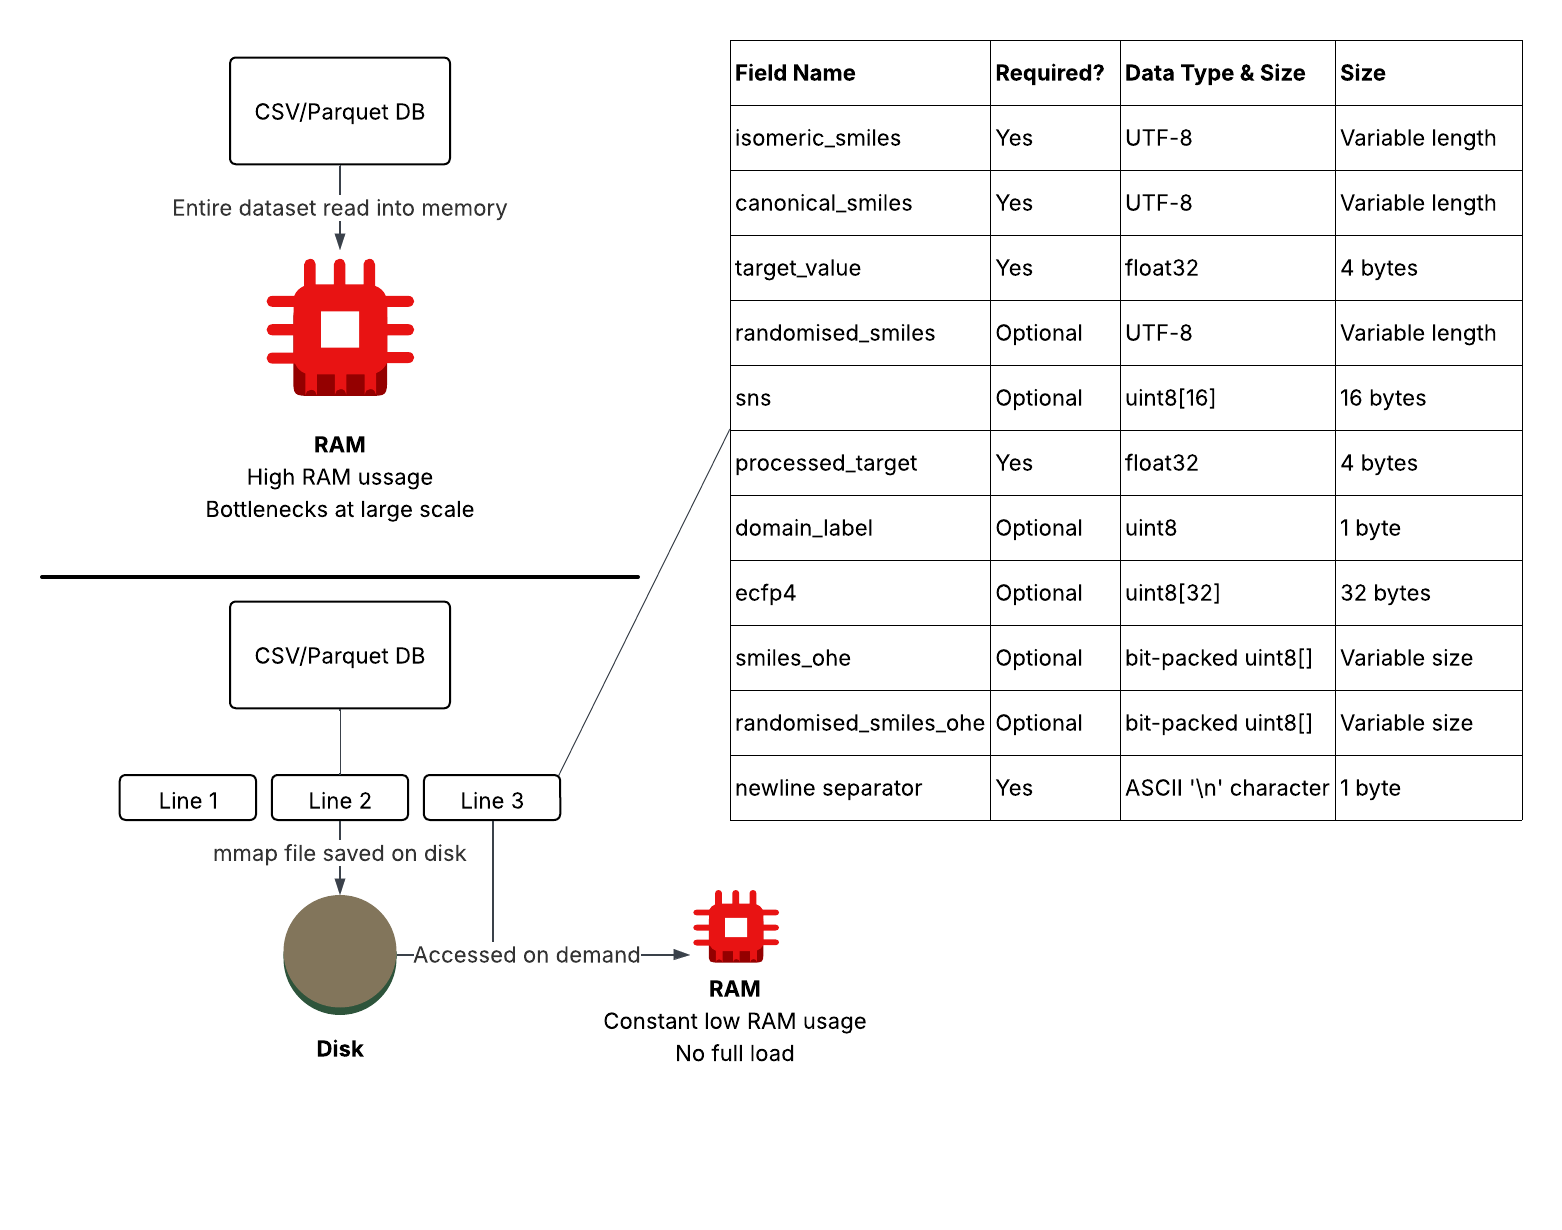
\includegraphics[width=0.95\textwidth]{figure_mmap_structure.png}
    \caption{Memory-mapped file architecture contrasted with traditional in-memory loading. Top: CSV/Parquet approaches load entire datasets into RAM, creating bottlenecks at scale. Bottom: Memory-mapped binary files enable on-demand line-by-line access with constant low RAM usage. Right: Entry-level structure showing byte-aligned fields with fixed-size representations (target values, fingerprints, domain labels) and length-prefixed variable-length fields (SMILES strings, one-hot encodings).}
    \label{fig:fig_mmap}
\end{figure}


\subsection{Uncertainty}
% ---- NOTES: Uncertainty ----
% Takeaway: how each model's uncertainty splits into an aleatoric and an epistemic part, and why comparisons with the injected noise use out-of-fold training molecules.
% - Change: "the variance the labels the molecule's given leaf" should read "the variance of the training labels in the molecule's leaf, in each tree". That is what the quantile regression forest computes, before averaging over the trees.
% - Change: "The total aleatoric uncertainty are those variances" should read "is".
% - Change: "the sum of the the aleatoric" has a doubled "the".
% ---- END NOTES ----

Up to this point we have been concerned with how noise affects the predictive accuracy of QSAR models. However, label noise should also affect the uncertainty these models report. Some models return only a point prediction, while others also return an estimate of uncertainty, either as a predicted distribution or as the spread across an ensemble. Furthermore, some report a single value of uncertainty while others report one that can be decomposed into an aleatoric and an epistemic component \citep{kendall2017}. The aleatoric component describes underlying noise the model associates with the data, while the epistemic component represents the uncertainty within the model's fit. We sought to determine if, as expected, the aleatoric component rises with injected label noise while the epistemic component does not.

For the BNN and VBLL transformations, we took the two components over $T = 100$ stochastic forward
passes \citep{kendall2017}:
\begin{equation}
\hat{u}^2_{\text{ale}}(x) = \frac{1}{T}\sum_{t=1}^{T}\hat{v}_t(x),
\qquad
\hat{u}^2_{\text{epi}}(x) = \frac{1}{T}\sum_{t=1}^{T}\big(\hat{\mu}_t(x) - \bar{\mu}(x)\big)^2 ,
\label{eq:sampling_split}
\end{equation}
where $\hat{\mu}_t(x)$ and $\hat{v}_t(x)$ are the mean and the variance returned for molecule $x$ on
pass $t$, and $\bar{\mu}(x)$ is the mean over passes. Here $\hat{v}_t(x)$ is the predicted observation
noise variance. It varies per molecule in the variance-head and heteroscedastic variants, and is one
number for the whole fit in the VBLL transformation. A full-BNN without a variance head returns no
variance, so its uncertainty is epistemic alone.

The other models follow the same split. For GPs, the epistemic component is the posterior variance of the latent function and the aleatoric component is the learned observation noise \citep{Rasmussen2005}. All variants of the GP produce one number for the whole fit except heteroscedastic. For QRF models, each tree holds multiple training molecules. So for a given molecule, the aleatoric component is the variance the labels the molecule's given leaf. The total aleatoric uncertainty are those variances averaged over the trees. The epistemic component is the variance of the leaf means across the trees. NGBoost predicts one variance for each molecule from a single fit, which is aleatoric alone \citep{Duan2020}. In every model, the total uncertainty is the sum of the the aleatoric and epistemic components.

No held-out label carries injected noise, so every comparison against the injected noise was made on
training molecules. Each training set was divided into five folds grouped on Murcko scaffolds, and each
molecule was scored by a refit that excluded its own fold. For NGBoost on QM9, three of the five folds
were scored to limit its cost. No uncertainty was calibrated after fitting.


\subsection{Evaluation}
% ---- NOTES: Evaluation ----
% Takeaway: robustness is AUC_norm, the normalised area under the R^2 retention curve, read beside clean R^2.
% Takeaway: an ANOVA per noise condition splits the variance between model and representation.
% Result needed: the excluded-configurations Additional file still uses the gate clean R^2 <= 0.6 in its caption and rows. Regenerate it at 0.3.
% Paragraph 4: rank correlations and the Wilcoxon test.
% - Change: "probabilistic models with its deterministic counterpart" should read "each probabilistic model with its deterministic counterpart".
% Paragraphs 5 to 7 below are out of date. Her current paper (Performance metrics) has all three rewritten in her words. Copy them in, citing each Additional file by its label.
% Paragraph 5: the ANOVA.
% - The model has a replicate block and a model-within-family term. It is no longer a plain two-way model.
% - Terms: replicate $s_r$, model family $\alpha_f$, model within family $\gamma_{m(f)}$, representation $\beta_j$, family x representation, model-within-family x representation, residual.
% - Type I sums of squares, entered in the order replicate, family, model within family, representation, interactions.
% - The uncertainty on each share is the 95% interval of $\eta^2$ over 1,000 bootstrap resamples of whole replicates. Leaving one replicate out is no longer used.
% - The shares describe the models and representations tested here, not model or representation choice in general.
% Paragraph 6: why models are grouped into families (replaces the correlation-exclusion text).
% - No model and no representation is dropped on a correlation. The rho > 0.99 model rule and the rho > 0.90 Sort & Slice rule come from an earlier version of the study.
% - Two things break independence. Each QM9 replicate shares one data split and one noise draw across all models, so the replicate enters as a block.
% - Near-identical versions of one method would count several times towards the model share. So models are grouped into families, and each model is nested in its family.
% - Grouping rule: the mean difference between two models is smaller than their replicate-to-replicate standard deviation in at least 16 of 24 comparisons.
% - The 24 comparisons are 4 outcomes (clean R^2, and AUC_norm under Gaussian, grouped-shifted and grouped-wider noise) on each of 6 representations.
% - Five pairs met the rule: RF with QRF (16 of 24), XGBoost with LightGBM (23 of 24), NN-alpha with BNN-alpha (20 of 24), NN-beta with BNN-beta (18 of 24), VBLL-alpha with VBLL-beta (20 of 24).
% - So the 13 base models form 8 families. Within a family, model differences explain at most 3.5% of the variance in any outcome and noise condition.
% - Tukey's HSD between family members, per representation, is reported beside each difference. It does not form the families.
% Paragraph 7: all six representations are kept (replaces the Sort & Slice exclusion and the ICC sentences).
% - ECFP4 and Sort & Slice were considered as one group, because both encode circular substructures.
% - Count per outcome: of the 13 base models, how many had the two representations closer than their replicate-to-replicate standard deviation.
% - Clean R^2: 0 of 13 models, differences 0.035 to 0.105. So all six representations stay as separate levels.
% - Under noise: 5 of 13 (Gaussian), 12 of 13 (grouped-shifted), 4 of 13 (grouped-wider). Clean R^2 decided it.
% - Change: drop the ICC(1,1) sentences. No current result depends on ICC.
% - Change: the model redundancy, representation redundancy and ICC Additional files hold numbers from the earlier study. Do not cite their numbers.
% - Cite instead three tables made for the paper: candidate model families (one row per pair of base models), candidate representation groups (ECFP4 with Sort & Slice), and Tukey's HSD within each family. They are not yet in the thesis appendix.
% Paragraph 8: the three uncertainty questions.
% - Change: "whether uncertainty rise" should read "rises"; "models who report" should read "models that report".
% - Change: the second question divides the epistemic rise by the mean aleatoric part. The results divide it by the rise in mean aleatoric uncertainty. Make the sentence say that.
% ---- END NOTES ----
We compute statistics on the held-out molecules, for QM9 the test split and for three assay datasets the held-out fold of the scaffold cross-validation. Different combinations of dataset, model, representation, noise condition, and noise level are examined in each scenario. We used the coefficient of determination ($R^2$) throughout. For molecule $i$, let $y_i$ be the clean label, $\hat{y}_i$ the prediction, $\epsilon_i$ the noise injected into its label and $u_i$ the predicted uncertainty.

To evaluate the effect of label noise, we tracked predictive performance retention under increasing artificial noise. For each QSAR pairing we recorded $R^2(\tau)$ at each noise level $\tau$, and normalized it to obtain the retention ratio $R^2(\tau)/R^2(0)$. To quantify robustness, we used the normalized area under this retention curve, \aucnorm (Equation~\ref{eq:auc_norm}), evaluated using the trapezoidal rule over the seven noise levels. While we tested other metrics of robustness, we found \aucnorm to be less directly correlated to clean-label $R^2$ predictions. For censoring, we sweep over a set of fractions to clip the labels prior to normalization. 

An \aucnorm value near 1 indicates that the QSAR model in question has retained predictive performance with artificial noise, meaning it is more robust to noise. Since we normalize the curve by its own clean-label predictive performance, a model with a low clean $R^2$ has less to lose, so \aucnorm is reported beside clean $R^2$. We excluded replicates with a clean $R^2 < 0.3$ from the robustness analysis (Additional file~\ref{app:noise:sec:excluded_configurations}), as performance retention ratios become unstable when the clean-label denominator approaches zero. On QM9 one \aucnorm is computed per replicate, and we report the median over the ten replicates. On the three assay datasets one value is computed per scaffold fold, and the median over the five folds is reported. 

To compare the relative effect of the thirteen base models across datasets and noise conditions, we compared their rankings using Spearman's rank correlation coefficient ($\rho$) between clean $R^2$ and \aucnorm. We compared probabilistic models  with its deterministic counterpart using a two-sided Wilcoxon signed-rank test paired on the replicate, at $\alpha = 0.05$, separately for each representation and noise condition. This test was run only on QM9, as with five scaffold folds the
smallest attainable $p$ is 0.0625.

We conducted a separate two-way analysis of variance (ANOVA) for each noise condition to identify the
relative contributions of molecular representation and model architecture to both predictive
performance and noise robustness. For a given metric $y$, either $R^2$ at a noise level of 1.0 or
\aucnorm:
\begin{equation}
y_{ijr} = \mu + \alpha_i + \beta_j + (\alpha\beta)_{ij} + e_{ijr},
\end{equation}
where $\alpha_i$ represents the effect of model architecture $i$, $\beta_j$ represents the effect of
molecular representation $j$, $(\alpha\beta)_{ij}$ is the interaction term, and $e_{ijr}$ is the
residual for replicate $r$. The proportion of variance explained by each term was calculated as the
effect size
\begin{equation}
\eta^2_{\text{term}} = \frac{SS_{\text{term}}}{SS_{\text{total}}},
\end{equation}
using Type I (sequential) sums of squares, entered in the order model architecture, molecular
representation, interaction. The ten QM9 replicates provide the residual. The uncertainty on each share is the range of $\eta^2$ when the decomposition is repeated with each replicate left out in turn. 

ANOVA relies on the assumption that observations both within and across groups are independence. Across the whole set of models and representations in this study, some pairs produced similar predictions that are not independent. This causes the residual degrees of freedom to increase, while the residual sum of squares barely moves. To handle this issue, we computed pairwise Spearman rank correlations between all models and between all representations across noise strategies. Models whose profiles correlated at $\rho > 0.99$ with another model were excluded, including quantile regression forests (QRF), which were very similar to RF, as well as different BNN variants. 

Across representations, SNS correlated at $\rho > 0.90$ with the ECFP4 fingerprint and was excluded to avoid inflating representation degrees of freedom, as both encode overlapping circular substructure information. We also computed intraclass correlation coefficients ICC(1,1) for all model pairs. ICC(1,1) measures the proportion of total variance attributable to between-subject differences, with values near 1.0 indicating that two models rank configurations almost identically. The full redundancy and ICC tables are reported in Additional files~\ref{app:noise:sec:model_redundancy}--\ref{app:noise:sec:model_icc}.

To assess the interaction between uncertainty estimation and label noise, we posed three questions. First, whether uncertainty rise with label noise, as measured by the mean $u_i$ over held-out molecules at the highest noise level
divided by its value with no added noise, in each replicate or fold. The second pertains to models who report separate aleatoric and epistemic components. We divided the increase of mean epistemic uncertainty between the highest level of noise and clean labels by the mean of the aleatoric component to determine how each responds to label noise. A ratio near 0 means the added noise was attributed to the labels while a ratio of 1 or above means the epistemic component grew as much or more. We also compared the mean aleatoric component with the standard deviation of the injected noise. The third question we had was whether per-sample uncertainty values track injected label noise, as measured by the Spearman correlation between $u_i$ and $|\epsilon_i|$ over out-of-fold training molecules, per fold and per noise level. We also report the Spearman correlation between $u_i$ and the absolute error of the prediction. Finally, we asked whether dividing a molecule's out-of-fold absolute error by $u_i$ ranks the corrupted labels better than the error alone, and report the difference between the two Spearman correlations with $|\epsilon_i|$.


\section{Representation governs clean performance, architecture governs robustness}
% ---- NOTES: Representation governs clean performance, architecture governs robustness ----
% Takeaway: model architecture explains most of the variance in noise robustness. For accuracy at a fixed noise level, model and representation are comparable.
% Takeaway: the model-by-representation interaction is larger for robustness than for accuracy.
% - Change: the prose, table and three figures below come from an earlier version of the study (six noise strategies, the noise degradation slope, a clean R^2 gate of 0.6). Rewrite them from the bullets below.
% Result needed: regenerate the variance-decomposition table and figure with the replicate block and the eight model families. Every share below will change.
% Paragraph 1: what was decomposed, and on what.
% - An ANOVA per noise condition splits the variance between model architecture, representation, their interaction and a residual.
% - Data: QM9 HOMO--LUMO gap, 13 base models x 6 representations x 10 replicates.
% - Three noise conditions, the ones run on every model and representation: Gaussian, grouped-wider, grouped-shifted.
% - Two outcomes: robustness as AUC_norm, and accuracy as R^2 at a noise level of 1.0 (one spread of the clean training labels).
% Paragraph 2: architecture dominates robustness; accuracy splits evenly.
% - Gaussian, R^2 at level 1.0: model 29.1%, representation 26.6%, interaction 13.7%, residual 30.6% of the variance.
% - Gaussian, AUC_norm: model 49.5%, representation 9.2%, interaction 20.4%, residual 20.8%.
% - Grouped-wider gives the same picture: AUC_norm model 50.5%, representation 8.6%; R^2 model 36.3%, representation 24.7%.
% - Reason given in the paper: label noise does not change the features, so the representation has little say in how a model copes with it.
% - Change: the prose says the interaction is the largest share of accuracy (46-49%). It is now 13.7% under Gaussian noise.
% Paragraph 3: the interaction term.
% - The interaction is larger for robustness than for accuracy: 20.4% against 13.7% of the variance, Gaussian noise.
% - It is about the size of the residual (20.8%).
% - Reading: some models depend on different sets of features, and label noise widens that difference.
% - Change: the earlier-study points on this interaction (SVM and BNN robust on every representation; model share of NDS variance 91% on SMILES against 72% on PDV; PDV with the shallowest NDS) are replaced by the AUC_norm decomposition. SMILES is not one of the six representations.
% Paragraph 4: grouped-shifted noise is dominated by the residual.
% - Grouped-shifted: residual 56.3% of the variance in AUC_norm and 76.6% in R^2.
% - Model architecture falls to 30.5% (AUC_norm) and 7.1% (R^2).
% - Reading: the offset drawn for each scaffold group differs between replicates, and that drives the variance.
% - The intervals are wide here: R^2 model share 7.1 +- 6.2%, residual 76.6 +- 13.6%.
% Paragraph 5: clean labels and the three assay datasets.
% Result needed: clean-label decomposition row (R^2 before any noise).
% Result needed: decomposition on LogD, Caco-2 and hERG K_i under AUC_norm. The Additional file on the assay-dataset ANOVA still shows NDS.
% Table (replaces the table below): one row per noise condition x outcome (6 rows: 3 conditions x AUC_norm, R^2 at level 1.0), plus the clean-label row.
% - Columns: model, representation, interaction, residual (eta^2, % of variance), then counts of models (13), representations (6), replicates (10).
% - Uncertainty on each share: the 95% interval over 1,000 bootstrap resamples of whole replicates.
% Figure (replaces the ANOVA figure below): panel a) AUC_norm, panel b) R^2 at level 1.0; x axis noise condition, y axis share of variance.
% - Change: the interaction figure (NDS heatmap; NDS on PDV against ECFP4, Spearman 0.73 over 11 models) has no current counterpart. Drop it or rebuild it on AUC_norm.
% - Change: the last paragraph and the global-overview figure compare clean performance with robustness per model. They move to that comparison, rewritten.
% - Their gate is out of date: exclusion is now clean R^2 < 0.3, per replicate on QM9 and per fold on the assay datasets.
% ---- END NOTES ----


Considering the two main components of a QSAR model, the molecular representation and the model architecture, we sought to understand how each contributes to predictive performance and noise robustness. ANOVA decomposition across six noise strategies on models to predict HOMO--LUMO gap from QM9 demonstrates that for predictive performance (R$^2$ at $\sigma = 0.3$), the model--representation interaction term is the  largest source of variance across all six strategies, followed by model architecture and representation (Table~\ref{tab:anova_decomposition}; Figure~\ref{fig:anova_decomposition}a). However, for noise robustness as measured by the noise degradation slope (NDS), this ordering shifts. The choice of model architecture is instead the largest source of variance, while the interaction term drops to second and representation third. This observed inversion makes sense because the molecular representation dictates the chemical information the model receives, while the architecture determines how efficiently that information is used. The interaction term reflects the idea that these two are not independent. In the context of label noise robustness, representation has less of an impact since the features are not corrupted by noise. Meanwhile, the model's regularization, ensembling, and uncertainty handling have a stronger impact on how it handles noise. 

The impact varied by type of noise, represented by noise strategy (Figure~\ref{fig:anova_decomposition}b). The strategies which degraded in performance the most, threshold and value-proportional, both corrupted label regions, forcing models to rely on their inductive biases. This translates to the model architecture explaining a significant portion of the variance. On the other hand, outlier noise only affects statistical outliers. For outlier noise, model and interaction effects were both smaller.

\begin{table}[htbp]
\centering
\caption{ANOVA variance decomposition by noise strategy on the QM9 HOMO--LUMO gap. Each cell reports $\eta^2$ (\%), the share of variance explained by that factor. Columns: \textbf{Model} = model architecture effect; \textbf{Rep} = molecular representation effect; \textbf{Inter.}\ = model$\times$representation interaction; \textbf{Resid.}\ = residual unexplained variance. ``Performance'' uses R$^2$ at $\sigma = 0.3$ as the outcome; ``Robustness'' uses the noise degradation slope (NDS). Bold entries highlight the dominant factor in each row.}
\label{tab:anova_decomposition}
\small
\begin{tabular}{lcccccccc}
\toprule
& \multicolumn{4}{c}{\textbf{Performance ($\eta^2$, \%)}} & \multicolumn{4}{c}{\textbf{Robustness ($\eta^2$, \%)}} \\
\cmidrule(lr){2-5} \cmidrule(lr){6-9}
\textbf{Strategy} & \textbf{Model} & \textbf{Rep} & \textbf{Inter.} & \textbf{Resid.} & \textbf{Model} & \textbf{Rep} & \textbf{Inter.} & \textbf{Resid.} \\
\midrule
Gaussian        & 24.6 & 22.8 & \textbf{48.1} &  4.5 & \textbf{48.7} &  8.2 & 11.9 & 31.2 \\
Quantile        & 25.1 & 22.4 & \textbf{46.9} &  5.6 & \textbf{47.9} &  6.8 & 14.9 & 30.4 \\
Threshold       & 25.0 & 21.2 & \textbf{48.0} &  5.8 & \textbf{48.0} & 10.1 & 28.0 & 13.9 \\
Heteroscedastic & 27.9 & 23.5 & \textbf{46.2} &  2.5 & \textbf{37.0} &  4.5 & 17.5 & 41.0 \\
Value-prop.     & 27.8 & 22.0 & \textbf{46.5} &  3.8 & \textbf{52.8} &  6.9 & 22.2 & 18.2 \\
Outlier         & 25.3 & 22.0 & \textbf{49.2} &  3.5 & 12.7 &  3.2 &  4.7 & \textbf{79.3} \\
\bottomrule
\end{tabular}
\end{table}

\begin{figure}[htbp]
    \centering
    \includegraphics[width=\textwidth]{fig2_anova_decomposition.png}
    \caption{ANOVA variance decomposition ($\eta^2$, \%) for a) predictive performance (R$^2$ at $\sigma=0.3$) and b) noise robustness, quantified by the noise degradation slope (NDS), by noise strategy. Lower (more negative) NDS indicates faster performance loss under noise.}
    \label{fig:anova_decomposition}
\end{figure}

The interaction between model architecture and representation is seen in Figure~\ref{fig:interaction}. While some model architectures, like SVM and full BNNs maintain consistent noise robustness scores across all representations, others like NN-$\beta$ display greater variation. Model robustness on one representation strongly predicts robustness on another (Spearman $\rho = 0.73$, $p = 0.007$ for ECFP4 vs PDV; 11 models). However, the scatter around the diagonal reflects the interaction term identified by the ANOVA. 

\begin{figure}[htbp]
\centering
\includegraphics[width=\textwidth]{fig_interaction.png}
\caption{Representation--model interaction effects on the QM9 HOMO--LUMO gap. a) Noise degradation slope (NDS) heatmap showing model robustness across representations under Gaussian noise; lower (more negative) NDS indicates faster degradation. ``N/A'' indicates configurations excluded due to baseline $R^2 < 0.6$ or kernel incompatibility (GP uses a Tanimoto kernel defined on binary vectors, which is incompatible with PDV). b) NDS on PDV versus ECFP4 fingerprint for each model under Gaussian noise, with Spearman correlation.}
\label{fig:interaction}
\end{figure}

We filtered out model--representation configurations with baseline predictive performance R$^2 < 0.6$, excluding 66 configurations where poor clean-data performance would produce misleadingly shallow degradation slopes (Additional file~\ref{app:noise:sec:excluded_configurations}). We evaluated all model architectures under increasing label noise on the PDV representation across six strategies, considering both predictive performance as measured by $R^2$ as well as the noise degradation slope (NDS). We observe that NDS varies substantially across architectures and noise strategies, as seen in Figure~\ref{fig:global_overview}. 

\begin{figure}[htbp]
\centering
\includegraphics[width=\textwidth]{fig1_global_overview.png}
\caption{Global overview of noise robustness on the QM9 HOMO--LUMO gap. a) Performance degradation curves (PDV, Gaussian noise) showing R$^2$ versus noise level $\sigma$ for representative models. b) Noise degradation slope (NDS) heatmap across all model architectures and noise strategies on PDV; lower (more negative) NDS indicates faster degradation under noise. The Tanimoto GP is absent because its kernel is incompatible with PDV (see Section~\ref{sec2}); a separate GP with an RBF kernel is included for PDV-specific analyses.}
\label{fig:global_overview}
\end{figure}

\section{Probabilistic models are no more noise-robust than deterministic ones}
% ---- NOTES: Probabilistic models are no more noise-robust than deterministic ones ----
% Takeaway: the Bayesian versions of the networks kept more AUC_norm than the plain networks on all four datasets, at a cost in clean R^2.
% Takeaway: whether QRF is less robust than RF is open until RF at 300 trees is compared with QRF.
% - Change: the prose below is from the earlier study. It pairs NN with VBLL, reports noise degradation slopes, and uses QM9 alone. Rewrite it from the bullets.
% Paragraph 1: what is compared, and why only these pairs.
% - Question: does a model that reports a distribution, not a point value, lose less R^2 as labels get noisier?
% - Three pairs of the same core model: NN-alpha against BNN-alpha, NN-beta against BNN-beta, and RF against QRF.
% - Each network is also compared with its Bayesian version plus a variance head.
% - A pair is only comparable if both share one setting. Each network and its Bayesian version were tuned to the same setting.
% - QRF uses 300 trees, so it is compared with an RF of 300 trees, not the 100-tree RF of the main tables.
% - VBLL is not one of the pairs. VBLL-alpha and VBLL-beta are base models of their own, ranked with the other models.
% - The GP is not a deterministic-probabilistic pair and stays out of this section.
% Paragraph 2: networks against their Bayesian versions.
% - Robustness is measured by AUC_norm, not by the noise degradation slope.
% - The Bayesian networks kept more AUC_norm than the plain ones, and lost some clean R^2, on all four datasets.
% - BNN-beta kept more AUC_norm than NN-beta in most representation and noise combinations on every dataset.
% - BNN-alpha did so in most combinations on Caco-2 and logD, and in about half on hERG K_i.
% - A network with a lower clean R^2 has less to lose, so AUC_norm is read beside clean R^2.
% Result needed: rank of each Bayesian network against the other model families at the highest noise level, to test whether it only had less to lose.
% Paragraph 3: the variance head, and RF against QRF.
% - The Bayesian network with a variance head runs at a different setting from its Bayesian base. So a difference between them cannot be put down to the variance head alone. Say so.
% Result needed: change in AUC_norm and in clean R^2, variance-head network minus its Bayesian base, per dataset.
% Result needed: change in AUC_norm and in clean R^2, QRF minus RF at 300 trees, per dataset.
% - Change: drop "QRF was significantly less robust than RF" until the matched comparison is in. That result compared the 100-tree RF with QRF at 300 trees, so the two differed in tree count as well as in the quantile step.
% Paragraph 4 (keep only if the re-run still shows VBLL failing on the learned embeddings):
% - The VBLL networks were unstable on the learned embeddings.
% - Change: mol2vec is no longer used. The six representations are ECFP4, Avalon, Sort & Slice, PDV, ChemBERTa and MHG-GNN.
% - Change: VBLL is no longer a counterpart pair, so this point belongs with the base-model results if it survives.
% - Change: the exclusion rule is now clean R^2 < 0.3 per QM9 replicate or assay fold, not R^2 < 0.6 per configuration.
% Result needed: number of VBLL replicates or folds excluded on ChemBERTa and MHG-GNN under the clean R^2 < 0.3 rule.
% Table (replaces the Wilcoxon table): one row per pair and noise condition, one column per representation.
% - Each entry: median change in AUC_norm, then median change in clean R^2 in brackets, counterpart minus base, over 10 replicates.
% - Mark an AUC_norm change with the same sign in all 10 replicates. Add a column saying whether the pair shares one setting.
% - QM9 only in the chapter; the logD, Caco-2 and hERG K_i versions go to the Additional files.
% - The table carries no p-values.
% Result needed: the QM9 table after the re-run.
% Figure 1 (replaces the NN-family figure): held-out R^2 against injected noise, one row per dataset, ECFP4, Gaussian noise. Columns: the NN-alpha family, the NN-beta family, and RF (300 trees) against QRF.
% Figure 2: change in AUC_norm (top row) and in clean R^2 (bottom row), counterpart minus base, per dataset. One mark per representation and noise condition.
% Result needed: Additional file~\ref{app:noise:sec:bayesian_transformation_tests} still reports slope-based Wilcoxon tests with VBLL pairs. Replace it with the per-representation AUC_norm changes.
% ---- END NOTES ----

To further explore the impact of model architecture on noise robustness, we examined variants of the same core architecture. Specifically, Bayesian transformations were used to explore the impact of the Bayesian framework on noise. By comparing models with the same core architecture, we observe that with full Bayesian transformations, representation explains less than $11\%$ of NDS variance ($p > 0.25$) while variational Bayesian inference on the same NNs is representation-dependent. On MHG-GNN and mol2vec representations, VBLL models were unstable, such that all 24 VBLL $\times$ \{MHG-GNN, mol2vec\} configurations were excluded due to baseline R$^2 < 0.6$. Further work could involve more thoroughly-tuning these models and exploring different core architectures to adapt to these embedding-style inputs. 

In general, the full Bayesian transformations reduced the degradation in performance with Gaussian noise the most, as seen in Figure~\ref{fig:nn_family_comparison}. Both full BNN and VBLL transformations significantly improved robustness for both NN-$\alpha$ and NN-$\beta$ (Table~\ref{tab:wilcoxon_bnn}). Full transformations are more computationally expensive, making VBLL a potentially stronger approach to handling noise with NNs when working with larger data sets or modeling architectures. The choice of transformation varies by representation, as seen in Additional file~\ref{app:noise:sec:bayesian_transformation_tests}, with SMILES receiving the largest benefits from Bayesian transformations. QRF was significantly less robust than RF (Table~\ref{tab:wilcoxon_bnn}), suggesting that quantile regression adds complexity and flexibility which may result in overfitting.

\begin{table}[htbp]
\centering
\caption{Wilcoxon signed-rank tests for Bayesian and probabilistic transformations on the QM9 HOMO--LUMO gap. \textbf{Base} is the deterministic reference model; \textbf{Variant} is the probabilistic/Bayesian transformation tested against it. \textbf{$\Delta$ NDS} = mean change in noise degradation slope (NDS) from base to variant; positive values mean the variant is more robust (slope closer to zero). \textbf{Sig.}\ marks pairs that are statistically significant at $p < 0.05$ (asterisk).}
\label{tab:wilcoxon_bnn}
\small
\begin{tabular}{llrrl}
\toprule
\textbf{Base} & \textbf{Variant} & \textbf{$\Delta$ NDS} & \textbf{$p$-value} & \textbf{Sig.} \\
\midrule
NN-$\alpha$ & BNN-$\alpha$ & $+0.056$ & $2.9 \times 10^{-10}$ & \textbf{*} \\
NN-$\alpha$ & VBLL-$\alpha$ & $+0.061$ & $1.2 \times 10^{-6}$ & \textbf{*} \\
NN-$\beta$ & BNN-$\beta$ & $+0.096$ & $2.9 \times 10^{-11}$ & \textbf{*} \\
NN-$\beta$ & VBLL-$\beta$ & $\mathbf{+0.124}$ & $1.2 \times 10^{-7}$ & \textbf{*} \\
RF  & QRF  & $\mathbf{-0.022}$ & $1.6 \times 10^{-10}$ & \textbf{*} \\
\bottomrule
\end{tabular}
\end{table}

\begin{figure}[htbp]
    \centering
    \includegraphics[width=\textwidth]{fig_nn_family_comparison.png}
    \caption{Neural network family comparison on the QM9 HOMO--LUMO gap with N=10k: R$^2$ versus $\sigma$ under Gaussian noise on the physicochemical descriptor vector (PDV) representation for a) NN-$\alpha$ family, b) NN-$\beta$ family, and c) RF versus QRF. Heteroscedastic results (not shown) are qualitatively consistent.}
    \label{fig:nn_family_comparison}
\end{figure}

\section{Relative model robustness is largely strategy-independent}
% ---- NOTES: Relative model robustness is largely strategy-independent ----
% Takeaway: clean accuracy does not predict robustness. The networks are among the most accurate on clean labels and the least robust; NGBoost the reverse.
% Takeaway: systematic noise costs more than random noise, and the shape of the noise distribution barely matters.
% Takeaway: the best representation for a model, and the order of the models, both change with the noise condition and the noise level.
% - Change: the prose and the table below come from the earlier study (six noise strategies, the noise degradation slope, 11 models). Rewrite them from the bullets below.
% - "Noise level" below is the noise added, as a multiple of the spread of the clean training labels.
% Paragraph A1: clean accuracy does not predict robustness.
% - Every model loses R^2 as noise grows. The loss stays small up to a noise level of about 0.5, then speeds up.
% - Across the thirteen base models, Gaussian noise, ECFP4: clean R^2 against AUC_norm has a Spearman correlation of -0.18 in the paper's text.
% Result needed: the latest results give -0.15. Recompute from the run the thesis reports.
% - A model with a low clean R^2 has less to lose, because AUC_norm divides by clean R^2. Say this once, here.
% Paragraph A2: by model family.
% - Forests, boosted trees, SVM and the GP: accurate on clean labels and robust.
% - The plain and Bayesian networks (NN-alpha, NN-beta, BNN-alpha, BNN-beta): among the most accurate on clean labels, NN-beta the most accurate at R^2 = 0.851.
% - They are also the four least robust (AUC_norm 0.881 to 0.897, ECFP4, Gaussian).
% - The two variational networks: lower clean R^2 (0.754 and 0.772) and middling robustness (AUC_norm 0.924 and 0.926).
% - NGBoost: the highest AUC_norm on all six representations under Gaussian noise. Its clean R^2 runs from 0.706 (ECFP4) to 0.865 (PDV); it is the least accurate model on four of the six.
% - On PDV it starts lowest in R^2 and ends highest, passing the other models between noise levels 1.0 and 1.5. On ECFP4 it stays lowest at every level.
% Paragraph A3: the representation matters more for the networks.
% - Under Gaussian noise, the six networks' AUC_norm spans more across the six representations than any other model's.
% Result needed: the paper's text gives the networks' span as 0.039 to 0.063, against at most 0.030 for every other model. The latest results give 0.037 (NN-alpha) to 0.069 (NN-beta), against at most 0.030 (QRF). Take the numbers from the run the thesis reports.
% - This is the model-level evidence for the interaction term in the variance decomposition.
% - Configurations excluded before any of this: clean R^2 < 0.3, per replicate on QM9 and per fold on the assay datasets.
% Floats for A1 to A3:
% - R^2 against noise level for the eight most robust base models (a: ECFP4, b: PDV).
% - Clean R^2 against AUC_norm, one point per base model (a: Gaussian, b: grouped-shifted).
% - AUC_norm grid, rows models, columns the six representations (a: Gaussian, b: grouped-shifted).
% Paragraph 1: how the conditions differ, and why the amount of noise is held fixed.
% - Five of the seven conditions draw each label's error on its own, so the error is random.
% - Grouped-shifted gives a whole scaffold group one shared offset. Censoring clips every label above a limit to that limit. Both are systematic.
% - Noise is added in proportion to the spread of the clean training labels, so two conditions differ in pattern, not amount.
% - Censoring cannot be held to a set amount: its levels are the fraction of labels clipped (0 to 0.5).
% - No table binning the conditions into mild, moderate and severe.
% Paragraph 2: the shape of the distribution makes little difference.
% - Gaussian against Laplace, Student-t and outlier noise, QM9 HOMO--LUMO gap, on the 21 pairings of model and representation these ran on.
% - SVM on PDV: AUC_norm 0.937 under Gaussian noise, against 0.947 (Student-t), 0.952 (outlier) and 0.955 (Laplace).
% - NGBoost lost AUC_norm under every non-Gaussian shape. It fits a per-molecule scale under a Gaussian likelihood, which the other shapes violate.
% - None of the 63 changes (21 pairings x 3 shapes) exceeds the spread across that pairing's ten replicates under Gaussian noise.
% - Agrees with \citet{Heid2023}: no difference between error distributions with a matched mean and standard deviation.
% Paragraph 3: systematic noise costs more than random noise.
% - Grouped-shifted lowered AUC_norm, relative to Gaussian noise, on 77 of the 78 pairings of base model and representation. The exception is BNN-beta on ECFP4 (0.871 to 0.873).
% - The loss is larger than that model's replicate spread on 50 of the 78 pairings.
% - It is within the spread on every representation for VBLL-alpha and VBLL-beta, and on five of six for BNN-alpha and BNN-beta.
% - The plain networks lost the most on every representation: up to 0.111 AUC_norm (NN-alpha, Avalon). The variational networks lost at most 0.033. RF lost 0.024 to 0.038.
% - Each Bayesian network lost less than its plain counterpart: BNN-beta on all six representations, BNN-alpha on five (on PDV the two lose 0.056 and 0.055).
% - Grouped-wider changed no model beyond its replicate spread, except QRF on Avalon and on MHG-GNN.
% - Censoring gave the largest drop: median AUC_norm 0.813, against 0.951 for the same five pairings under Gaussian noise.
% Paragraph 4: the best representation for a model depends on the noise condition.
% - From Gaussian to grouped-shifted, five of the thirteen base models change their best representation.
% - NGBoost Avalon to PDV; SVM ChemBERTa to ECFP4; NN-alpha PDV to ChemBERTa; BNN-alpha PDV to MHG-GNN; BNN-beta PDV to ChemBERTa.
% Result needed: confirm the fifth model. The paper's text gives NN-beta (PDV to Sort & Slice); the latest results give BNN-beta, with NN-beta best on ChemBERTa under both conditions.
% - Some of these are narrow: NGBoost's Gaussian best, Avalon (0.982), is 0.002 AUC_norm ahead of ChemBERTa. Give the gap beside each change.
% - So a representation chosen under one assumption about the noise is not necessarily the best under another.
% Paragraph 5: model ranks move with the noise level.
% - ECFP4, Gaussian: six of the seven most robust models start within 0.015 of one another in clean R^2 (0.830 to 0.845).
% - They stay together up to a noise level of 0.5 and separate only above 1.0. At noise level 1.5 they finish between 0.693 (LightGBM) and 0.741 (RF) R^2.
% Result needed: the paper's text gives LightGBM 0.693 at noise level 1.5; the latest results give 0.692. Take the number from the run the thesis reports.
% - Ranked by R^2 at each level among the thirteen base models: RF goes from seventh on clean labels to first by level 1.0. SVM goes from first to fourth.
% - AUC_norm weights levels 0 to 1.5 equally, and the lower half separates the models little. So it can understate what the pattern of the noise costs.
% - Reporting R^2 at one level has its own drawback: ranks shift at a different pace under each condition.
% Table: the change in AUC_norm from Gaussian to grouped-shifted noise, QM9. One row per base model (13 rows); negative is a loss.
% - Columns: one per representation (6), the replicate spread, then a count of representations on which the loss exceeds that spread.
% - Replicate spread: highest minus lowest AUC_norm across the ten replicates under Gaussian noise, for that model on that representation. The column gives its range over the six representations (e.g. RF 0.013 to 0.022).
% Figure: AUC_norm under every condition on the pairings the non-Gaussian shapes and censoring ran on, QM9. Panels a) ECFP4, b) PDV, c) ChemBERTa; rows models, columns conditions, Gaussian first.
% Figure: RF R^2 against noise level, one line per condition, QM9, ECFP4. Censoring has no line.
% Figure: rank of each base model against noise level, QM9, ECFP4. Panel a) Gaussian, b) grouped-shifted; median rank over ten replicates.
% - Change: drop the NDS table, Kendall's W = 0.92 and the NDS spread by strategy (0.06 outlier, 0.23 threshold). The current study has no counterpart.
% - Change: threshold, quantile, heteroscedastic and value-proportional noise are not among the seven conditions.
% - Change: the ANOVA, interaction and SMILES/PDV variance-share paragraphs are replaced by the variance decomposition on AUC_norm. SMILES is not among the six representations.
% - Change: the Gaussian top-10 configurations paragraph uses NDS. Drop it or rebuild it on AUC_norm.
% - Change: the two Additional files cited in the first paragraph (ECFP4 overview; clean R^2 against robustness) are from the earlier study and need regenerating on AUC_norm.
% ---- END NOTES ----

NGBoost and SVM showed the smallest degradation in predictive performance across all strategies, while NN-$\beta$ showed the steepest (Table~\ref{tab:nds_ranking}). When sorting models by NDS, their ranks across noise strategies were consistent: Kendall's $W = 0.92$ ($p = 2.7 \times 10^{-8}$; 11 models, 6 strategies), indicating that a model's relative robustness is largely strategy-independent. The same ranking pattern holds on the ECFP4 fingerprint (Additional file~\ref{app:noise:sec:ecfp4_overview}). Robustness is also largely decoupled from baseline predictive performance: across models on PDV under Gaussian noise, NDS clusters near $-0.38$ regardless of baseline R$^2$ (Additional file~\ref{app:noise:sec:clean_r2_vs_robustness}), so a high-performing model is not automatically a more robust one.

\begin{table}[htbp]
\centering
\caption{Noise degradation slope (NDS) by model on PDV (QM9 HOMO--LUMO gap), ranked by mean across six strategies. Lower $|$NDS$|$ (slope closer to zero) indicates greater robustness. Strategy abbreviations: \textbf{Gauss.}\ = Gaussian, \textbf{Quant.}\ = Quantile, \textbf{Thresh.}\ = Threshold, \textbf{Hetero.}\ = Heteroscedastic, \textbf{Val.-P.}\ = Value-Proportional. Bold rows mark the two most robust models; bold cell entries mark each strategy's most robust configuration.}
\label{tab:nds_ranking}
\small
\begin{tabular}{lccccccc}
\toprule
\textbf{Model} & \textbf{Gauss.} & \textbf{Outlier} & \textbf{Quant.} & \textbf{Thresh.} & \textbf{Hetero.} & \textbf{Val.-P.} & \textbf{Mean} \\
\midrule
\textbf{NGBoost}    & $\mathbf{-0.33}$ & $-0.12$ & $\mathbf{-0.29}$ & $\mathbf{-0.65}$ & $\mathbf{-0.18}$ & $\mathbf{-0.58}$ & $\mathbf{-0.36}$ \\
\textbf{SVM}        & $-0.36$ & $\mathbf{-0.11}$ & $-0.30$ & $-0.71$ & $-0.20$ & $-0.63$ & $-0.38$ \\
RF                  & $-0.36$ & $-0.12$ & $-0.30$ & $-0.71$ & $-0.20$ & $-0.63$ & $-0.39$ \\
LightGBM            & $-0.36$ & $-0.13$ & $-0.32$ & $-0.72$ & $-0.20$ & $-0.64$ & $-0.40$ \\
VBLL-$\alpha$       & $-0.38$ & $-0.16$ & $-0.35$ & $-0.68$ & $-0.22$ & $-0.60$ & $-0.40$ \\
XGBoost             & $-0.37$ & $-0.13$ & $-0.33$ & $-0.72$ & $-0.20$ & $-0.65$ & $-0.40$ \\
VBLL-$\beta$        & $-0.39$ & $-0.14$ & $-0.34$ & $-0.70$ & $-0.23$ & $-0.64$ & $-0.41$ \\
BNN-$\alpha$        & $-0.38$ & $-0.15$ & $-0.35$ & $-0.72$ & $-0.21$ & $-0.64$ & $-0.41$ \\
BNN-$\beta$         & $-0.38$ & $-0.15$ & $-0.36$ & $-0.72$ & $-0.21$ & $-0.65$ & $-0.41$ \\
NN-$\alpha$         & $-0.41$ & $-0.16$ & $-0.37$ & $-0.77$ & $-0.23$ & $-0.68$ & $-0.44$ \\
NN-$\beta$          & $-0.49$ & $-0.17$ & $-0.42$ & $-0.88$ & $-0.26$ & $-0.79$ & $-0.50$ \\
\bottomrule
\end{tabular}
\end{table}

The strategies differed not only in predictive performance severity, but also in their ability to discriminate between architectures. The spread of NDS across models differed by noise strategy, with outlier noise having a spread of 0.06 and threshold noise having 0.23, presumably exposing architectural differences that are masked by other types of noise. As seen in Table~\ref{tab:nds_ranking}, NGBoost was the most resistant to noise across strategies. With respect to the Variational Bayesian Last Layer (VBLL) models, VBLL-$\alpha$ showed a similar pattern, outperforming all tree-based models except NGBoost under threshold and value-proportional noise despite ranking below them under Gaussian noise. This suggests that its learned noise variance is most beneficial when label corruption is systematic rather than uniform. This observation with VBLL is not alone; predictive performance on clean data is not well-correlated with noise robustness. In fact, some of the models with the lowest NDS across strategies such as NGBoost and SVM did not perform particularly well on clean data. These models may be more prone to picking up on noise rather than underlying signals in the data. 

% TODO: review, needs manual review
As established by the ANOVA, model architecture and the model--representation interaction term dominate NDS variance. A handful of models stood out as being noise-robust regardless of representation, namely SVM and full BNNs. Both methods rely on inductive biases, SVM on margin maximization and BNN on weight priors. However, other models like RF and NN-$\beta$ show the opposite pattern. These models can be robust to noise, but only when paired with particular representations. The pairings differ by model. 

% TODO: review, needs manual review
While representation may not be a dominant determinant in NDS variance, the model--representation interaction term does have an impact. For SMILES, model choice explains over 91\% of robustness variance, while on PDV, model choice explains 72\%. Across all six noise strategies, PDV configurations produced the shallowest mean NDSs across representations, with its best performance coming with models with strong inductive biases like SVM and full BNN. This suggests that PDVs are preferable when dealing with noisy data. It appears that PDV's compact feature space complements margin-based and Bayesian regularization. Embeddings struggled, particularly when paired with NNs. These patterns are aligned with the importance of the model--representation interaction term, indicating that representation choice modulates noise robustness within a given architecture. 

Taking a closer look at model choice for noise robustness, we ranked all model--representation configurations on QM9 by their Gaussian NDS. Tree-based ensembles dominate the top 10: NGBoost appears five times, XGBoost and RF twice each, and LightGBM once. No neural-network configuration appears the top 10. Rankings are consistent across strategies and the top QM9 configurations maintain their advantage on ADME datasets, though SVM configurations rank higher on these ADME datasets than NGBoost.

\section{The pattern holds across prediction targets}
% ---- NOTES: The pattern holds across prediction targets ----
% Takeaway: on measured labels, RF keeps its QM9 standing; NGBoost, the boosted trees and VBLL-alpha do not.
% Takeaway: grouped-shifted noise is the hardest condition on every dataset, and the shape of the noise matters for SVM and NGBoost but not for RF or the GP.
% - Change: the prose below is from the earlier study. It reports NDS, NGBoost first everywhere, and heatmaps the current results replace. Rewrite it from the bullets below.
% - Rankings are for AUC_norm under Gaussian noise among the thirteen base models, at each of the six representations, unless a bullet says otherwise. Rank 1 is the most robust.
% Paragraph 1: what changes when the labels are measured, not computed.
% - The same noise injection is repeated on LogD and Caco-2 efflux \citep{openadmet} and hERG K_i \citep{Zdrazil2023}.
% - Change: the second figure's caption says hERG K_i has 1,482 molecules. The current dataset has 1,415 molecules.
% - These labels already carry measurement error in training and test labels. Injected noise adds to an unknown noise floor.
% - Repeat pK_i measurements of one compound disagree by about 0.54 log units \citep{Kalliokoski2013, Kramer2012}.
% - The hERG K_i labels have a spread of 0.915 log units. A noise level of 0.6 of the spread is about one unit of that laboratory error.
% - Robustness is AUC_norm, as on QM9. NDS is no longer used.
% Paragraph 2: clean labels, architecture against representation.
% - Share of the variance in clean R^2 (eta^2, %), 13 base models x 6 representations, per dataset:
%   Caco-2: model 36.2, representation 9.9, interaction 8.9, residual 44.9 (5 folds).
%   hERG K_i: model 33.4, representation 6.7, interaction 14.3, residual 45.6 (5 folds).
%   LogD: model 66.8, representation 16.8, interaction 9.5, residual 6.9 (5 folds).
%   QM9: model 39.1, representation 29.2, interaction 10.6, residual 21.1 (10 replicates).
% - So on clean labels the model term leads on all four datasets. Representation takes a smaller share on the assay datasets (6.7 to 16.8%) than on QM9 (29.2%).
% - On Caco-2 and hERG K_i almost half the clean-R^2 variance is residual, which here means fold-to-fold differences.
% - For comparison, on QM9 under Gaussian noise the AUC_norm split is model 47.8%, representation 8.1%.
% Result needed: the AUC_norm variance decomposition on the three assay datasets. The Additional file on the assay-dataset ANOVA is from the earlier study and must be regenerated before it is cited.
% Paragraph 3: the shape of the noise.
% - Laplace, Student-t and outlier noise were run on four base models (RF, the GP, SVM, NGBoost) and three of their variants, at ECFP4, PDV and ChemBERTa only.
% - Changes below are AUC_norm under each shape minus AUC_norm under Gaussian noise, same model and representation.
% - RF and the GP never lose more than 0.031 under these three or under grouped-wider noise, on any dataset.
% - SVM never loses under any of the four and gains up to 0.10 on the assay datasets (hERG K_i, grouped-wider).
% - NGBoost loses under all four on hERG K_i at every representation, by up to 0.12.
% - On Caco-2 NGBoost loses under all four, by up to 0.15, except grouped-wider at Avalon (+0.011).
% - So the shape of the added noise changes the outcome for SVM and NGBoost, not for RF or the GP.
% Result needed: a small table, per dataset, of the AUC_norm change under each shape for these four models.
% Paragraph 4: systematic noise.
% - Grouped-shifted noise gives the lowest median AUC_norm on every dataset, among the conditions that rank every model.
% - Grouped-shifted: Caco-2 0.733, hERG K_i 0.748, LogD 0.829, QM9 0.896. Gaussian: 0.826, 0.843, 0.877, 0.935.
% - No one model leads under grouped-shifted noise. RF ranks 1st to 4th on hERG K_i and LogD and 3rd to 8th on Caco-2. SVM ranks 3rd to 10th on the assay datasets.
% - NGBoost at ECFP4 has lower AUC_norm under grouped-wider than under grouped-shifted noise on Caco-2 (0.731 against 0.815) and hERG K_i (0.748 against 0.770).
% - This holds at 2 of 6 representations on Caco-2 and 1 of 6 on hERG K_i. Do not state it as general.
% - Censoring ran on a named subset of model-representation pairs, so it cannot rank models and is left out of figure (a).
% Paragraph 5: which model rankings carry over from QM9.
% - Open with: RF keeps its QM9 standing on the assay datasets; NGBoost, the two boosted-tree models and VBLL-alpha do not.
% - RF: 2nd on QM9 at five of six representations, and never below 7th on any assay dataset.
% - The GP: highest clean R^2 at most representations on the assay datasets, but only 3rd to 9th for AUC_norm. Accuracy and robustness rank it differently.
% - NGBoost: 1st on QM9 at every representation, as low as 10th on Caco-2.
% - LightGBM and XGBoost: near the bottom on Caco-2 and hERG K_i (LightGBM 10th to 13th), although LightGBM's clean R^2 ranks as high as 1st there.
% - VBLL-alpha: 1st or 2nd on hERG K_i, last on LogD. The dataset decides its standing.
% - The BNNs do not fall as a group. Change: drop "BNN variants suffer the most".
% - Say once that some representations on Caco-2 and hERG K_i rank 11 or 12 models, not 13, because models with clean R^2 < 0.3 are excluded.
% Table: rank ranges, one row per base model, one column per dataset, each cell the lowest to highest AUC_norm rank over the six representations. Next to ranking figure (b). Rows:
%   RF: QM9 2nd (3rd at PDV); LogD 1st at five of six; every assay dataset 1st to 7th.
%   GP (RBF kernel): assay datasets 3rd to 9th; clean R^2 1st at 6 of 6 on LogD, 5 of 6 on Caco-2, 4 of 6 on hERG K_i, 2nd otherwise.
%   NGBoost: QM9 1st; LogD 1st to 3rd; Caco-2 2nd to 10th; hERG K_i 6th to 9th.
%   LightGBM: Caco-2 and hERG K_i 10th to 13th; LogD 5th to 11th; clean-R^2 rank 2nd to 9th on Caco-2, 1st to 8th on hERG K_i.
%   XGBoost: QM9 3rd to 8th; LogD 5th to 10th; Caco-2 10th to 12th; hERG K_i 11th to 12th.
%   VBLL-alpha: hERG K_i 1st or 2nd; LogD 13th at every representation (its clean R^2 is also last there).
%   VBLL-beta: LogD 12th at every representation; Caco-2 1st to 4th.
%   BNN-alpha: 2nd to 12th on QM9 and on each assay dataset.
%   BNN-beta: QM9 11th to 13th; assay datasets 3rd to 12th.
% Result needed: a table or figure for a representation other than ECFP4. The LightGBM and representation claims have no figure behind them yet.
% Paragraph 6: the RF against QRF sentence.
% - Change: "QRF was consistently less robust than RF on every external data set" does not hold. It compared RF at 100 trees with QRF at 300 trees.
% - RF at 300 trees against QRF, over 6 representations x 3 noise conditions (Gaussian, grouped-wider, grouped-shifted) per dataset: QRF has the higher AUC_norm in 10 of 18 on Caco-2, 4 of 18 on hERG K_i and 3 of 18 on LogD.
% - Under grouped-shifted noise QRF is lower at every representation on all three datasets. Under grouped-wider it is higher at every representation on Caco-2.
% Result needed: confirm the RF (300 trees) against QRF numbers once the paper includes them.
% Result needed: the assay AUC_norm decomposition by representation, before claiming representation has a minimal effect on robustness on the assay datasets.
% Figures: both current figures report NDS and must be replaced.
% - (a) AUC_norm per model x noise condition on ECFP4, one panel per assay dataset, clean R^2 as the first column, thirteen base models as rows (Gaussian, grouped-wider, grouped-shifted).
% - (b) Rank for AUC_norm of each base model on QM9 and on each assay dataset, ECFP4, Gaussian noise; rows are models.
% ---- END NOTES ----

\begin{figure*}[htbp]
\centering
\includegraphics[width=\textwidth]{fig_validation_overview.png}
\caption{Noise degradation slope (NDS) heatmaps for three external validation datasets: a) LogD, b) Caco-2 Efflux, and c) hERG K$_i$. Lower (more negative) NDS indicates faster degradation under noise. Black cells indicate baseline R$^2 < 0.3$ for that (model, strategy) pair; ``N/A'' indicates filtered extreme values ($|$NDS$| > 2$). Models whose baseline R$^2$ fell below 0.3 across all strategies are omitted entirely, accounting for the smaller set of rows on hERG K$_i$.}
\label{fig:validation_overview}
\end{figure*}

In addition to working with ``clean'' quantum molecular properties, we tested our findings on experimentally-obtained data, replicating our process of adding artificial noise. Unlike QM9, where $\sigma = 0$ corresponds to a noise-free baseline, the experimental endpoints carry their own measurement noise in both training and test labels; the injected $\sigma$ therefore stacks on top of an unknown noise floor. Per-dataset NDS heatmaps across all model architectures and noise strategies are shown in Figure~\ref{fig:validation_overview}. The ANOVA on these additional datasets confirms that model architecture dominates robustness variance on all three datasets, as seen in Additional file~\ref{app:noise:sec:assay_variance_decomposition}, and that the trends with respect to noise robustness generalize. NGBoost ranks first on both QM9 and external datasets, SVM also transfer quite well. Some models' predictive capabilities are limited on these external datasets, likely due to a combination of smaller training sets, narrower chemical coverage, and the unknown experimental noise in the labels. XGBoost and BNN variants suffer the most here, as seen in Figure~\ref{fig:validation_combined}a.

\begin{figure*}[htbp]
\centering
\includegraphics[width=\textwidth]{fig_validation_combined.png}
\caption{Comparison of noise robustness on QM9 (HOMO--LUMO gap, $N = 10{,}000$) and three external validation datasets: LogD ($N = 5{,}039$), Caco-2 Efflux ($N = 2{,}161$), and hERG K$_i$ ($N = 1{,}482$). a) Model robustness measured by the noise degradation slope (NDS) across all four datasets; lower (more negative) NDS indicates faster degradation under noise. b) QM9 vs external robustness: models with inherent robustness mechanisms (NGBoost, SVM) maintain their relative standing, while ensemble-dependent models (XGBoost) degrade on the external datasets.}
\label{fig:validation_combined}
\end{figure*}

QRF was consistently less robust than RF on every external data set (Additional file~\ref{app:noise:sec:rf_vs_qrf_assay}). As seen with QM9, choice of molecular representation has a minimal effect on noise robustness across all three external datasets, reinforcing the finding that model architecture, not representation, is the main driver of noise robustness. 

\section{Uncertainty under label noise}\label{sec:uq}
% ---- NOTES: Uncertainty under label noise ----
% Takeaway: for the models that report uncertainty, this section asks whether it rises with label noise, and whether it points to the corrupted labels.
% Paragraph 1: the question.
% - The sections above measured how much accuracy each model keeps as labels get noisier.
% - Does mean predicted uncertainty rise as injected label noise rises?
% - Does a molecule's predicted uncertainty point to whether its own label was corrupted?
% - Change: end the existing paragraph with these two questions.
% Paragraph 2: what earlier comparisons of uncertainty methods on molecules found.
% - Hirschfeld et al. compared several neural-network uncertainty methods on five molecular regression benchmarks \citep{Hirschfeld2020}.
% - None of the methods was better than all others, and none ranked errors reliably across datasets \citep{Hirschfeld2020}.
% - Scalia et al. compared MC-dropout, deep ensembles and bootstrapping with graph networks on QM9 \citep{Scalia2020}.
% - Ensembles and bootstrapping beat MC-dropout; their framework also splits uncertainty into aleatoric and epistemic parts \citep{Scalia2020}.
% - Conformal prediction gives QSAR prediction ranges with a chosen error rate, as an alternative to an applicability domain \citep{Norinder2014}.
% - None of these injects label noise. That gap is what this section fills.
% Paragraph 3: a short map of the subsections, one sentence each, no numbers.
% - Mean uncertainty rises with noise. A molecule's own uncertainty does not rise with the noise on its own label, except under censoring, where it runs the other way.
% - How each model absorbs large residuals.
% - Whether the rise goes to the aleatoric or the epistemic part, and how the representation changes that.
% - The representation matters more for the uncertainty split than for robustness.
% ---- END NOTES ----
\todo[inline, color=yellow!40]{Write the opening of Section~\ref{sec:uq}. Hirschfeld, Scalia and Norinder are cited in no source -- add to refs.bib.}

The sections above showcased the importance of model selection when working with noisy labels. We take this one step further and ask, for the models which produce uncertainty estimates, how those estimates are affected by noise and if they can be used to track noise. 

\subsection{Models with an explicit noise term track prediction error under noise}
% ---- NOTES: Models with an explicit noise term track prediction error under noise ----
% Takeaway: mean predicted uncertainty rises with label noise, but per molecule it does not track the injected noise.
% Takeaway: censoring is the one exception, and there the sign is negative: the clipped labels get the lowest uncertainty.
% - Change: the prose and table below say per-molecule uncertainty tracks the injected noise. Computed within one noise level, it does not.
% Paragraph 1: the population-level result holds \citep{Kolmar2021}.
% - Mean predicted uncertainty rises with Gaussian label noise for every model and representation on QM9.
% - On the three assay datasets there are exceptions, all networks on learned embeddings.
% - BNN-alpha fails to rise in at least one fold on every assay dataset and representation.
% - Both full BNNs with a variance head fail on MHG-GNN for hERG K_i and Caco-2.
% - Table: mean predicted uncertainty at no added noise and at the highest noise level (PDV, Gaussian noise, held-out molecules).
% Result needed: the numbers for that table.
% Paragraph 2: per molecule, uncertainty does not track the injected noise under six of the seven noise conditions.
% - Measure: Spearman correlation, over test-set molecules, between predicted uncertainty and the size of the injected noise.
% - Compute it within one noise level. Pooling noise levels gives a large positive value only because uncertainty and noise both rise with the noise level.
% - Change: the 0.56 for GP on SNS in the table below is this pooled value. Within one noise level the same pair gives -0.04, at noise level 0.3 and at 0.6.
% - NGBoost on SNS: 0.47 pooled, 0.08 within noise level 0.3, 0.09 within noise level 0.6.
% - Why: Gaussian, Laplace, Student-t and grouped-shifted noise draw every label's noise from one scale. Outlier noise picks a random tenth of molecules. Grouped-wider holds each scaffold family in one fold.
% - Result: under these six conditions the correlation stays between -0.16 and 0.16 for every model, representation, dataset and noise level.
% Paragraph 3: censoring is the one case where tracking is possible, and the sign is negative.
% - Under censoring the noise depends on the label's value, so there is something to find.
% - QM9, half the labels clipped, PDV: -0.84 to -0.80 across folds for NGBoost; -0.47 to -0.41 for the GP.
% - logD: every fold of every model except the two GPs is at -0.29 or lower.
% - Error divided by uncertainty per molecule: the clipped labels are the ones the models are most certain about.
% - Consequence: low uncertainty could flag clipped molecules.
% Table: replace the table below. It pools noise levels and is from the earlier study (SNS, Morgan and mol2vec rows).
% - Replacement: uncertainty statistics per model and noise condition, QM9, PDV.
% - Columns: the slope of mean uncertainty against added noise, the rank correlation between uncertainty and error, and the change in how well corrupted labels are ranked.
% - The pooled correlation column goes.
% ---- END NOTES ----

\citet{Kolmar2021} found that the mean predicted uncertainty derived from the GPs increases with the amount of label noise in the training data. We go beyond the population level and instead ask if a model's per-sample uncertainty tracks label noise. One key sign that a model is able to handle noise is its ability to track it, represented by the per-sample Spearman correlation between predicted uncertainty and noise magnitude (Table~\ref{tab:top_unc_noise}). While GPs and NGBoost gave the strongest correlations, BNNs were moderate. Learned embeddings (MHG-GNN and mol2vec) struggled, so much so that their correlations dropped to near zero or below on every model tested. 

\begin{table}[htbp]
\centering
\caption{Strongest and weakest model--representation combinations for uncertainty--noise correlation on the QM9 HOMO--LUMO gap (Gaussian noise strategy). Columns: \textbf{Unc-Noise $\rho$} = Spearman correlation between predicted uncertainty and injected noise magnitude $|\epsilon|$ (higher = better noise detection); \textbf{Unc-Error $\rho$} = Spearman correlation between predicted uncertainty and absolute prediction error; \textbf{ECE} = expected calibration error (lower = better-calibrated); \textbf{Cov.\ $1\sigma$} / \textbf{$2\sigma$} = empirical coverage at the $1\sigma$ (68\% target) and $2\sigma$ (95\% target) intervals.}
\label{tab:top_unc_noise}
\small
\begin{tabular}{llrrrrr}
\toprule
\textbf{Model} & \textbf{Rep.} & \textbf{Unc-Noise $\rho$} & \textbf{Unc-Error $\rho$} & \textbf{ECE} & \textbf{Cov. $1\sigma$} & \textbf{Cov. $2\sigma$} \\
\midrule
\textbf{GP}    & \textbf{SNS}    & \textbf{0.56} & 0.23 & 0.14 & 71.2\% & 94.6\% \\
GP             & Morgan          & 0.53 & 0.22 & 0.14 & 71.4\% & 95.4\% \\
\textbf{NGBoost} & \textbf{SNS}  & \textbf{0.47} & 0.16 & 0.13 & 69.3\% & 95.4\% \\
\textbf{NGBoost} & \textbf{PDV}  & \textbf{0.47} & \textbf{0.29} & \textbf{0.11} & 69.0\% & 95.2\% \\
NGBoost        & PDV (binary)    & 0.44 & 0.25 & 0.13 & 69.8\% & 95.4\% \\
NGBoost        & Morgan          & 0.44 & 0.20 & 0.14 & 69.8\% & 95.3\% \\
BNN-$\alpha$   & SNS             & 0.42 & 0.21 & 0.17 & 73.4\% & 95.1\% \\
BNN-$\beta$    & SNS             & 0.40 & 0.21 & 0.18 & 73.5\% & 95.1\% \\
BNN-$\beta$    & Morgan          & 0.38 & 0.20 & 0.18 & 72.1\% & 95.0\% \\
BNN-$\beta$    & PDV             & 0.38 & 0.24 & 0.19 & 72.1\% & 94.0\% \\
\midrule
\multicolumn{7}{l}{\textit{Contrast: lowest correlations (graph/embedding representations)}} \\
\midrule
BNN-$\beta$ & mol2vec & $-0.05$ & 0.02 & 1.33 & 50.6\% & 76.4\% \\
VBLL-$\alpha$ & MHG-GNN & $-0.05$ & 0.09 & 13.41 & 26.6\% & 38.6\% \\
VBLL-$\beta$ & MHG-GNN & $-0.03$ & 0.10 & 15.34 & 31.1\% & 47.1\% \\
VBLL-$\beta$ & mol2vec & $-0.03$ & 0.15 & 23.86 & 44.8\% & 58.0\% \\
\bottomrule
\end{tabular}
\end{table}

\subsection{NGBoost and the GP stay near target coverage while Bayesian variants miscalibrate}
% ---- NOTES: NGBoost and the GP stay near target coverage while Bayesian variants miscalibrate ----
% Takeaway: each model absorbs the large residuals of noisy labels in its own way, and that decides where its uncertainty comes from.
% Paragraph 1: how each model handles large residuals (her paragraph below).
% - NGBoost predicts a scale per molecule, which grows to absorb a residual \citep{Duan2020}.
% - A GP with one global observation-noise term does not absorb single residuals \citep{Rasmussen2005, Obrezanova2007}.
% - The study also has a heteroscedastic GP, whose noise term depends on the input. Her paragraph describes only the global-noise GP.
% - BNNs broaden their weight posteriors instead \citep{gal2016, kendall2017}. VBLL learns one noise value for the whole fit \citep{Harrison2024}.
% - So VBLL's per-molecule uncertainty is epistemic only. It is not among the models whose uncertainty is split into aleatoric and epistemic parts.
% Paragraph 2: corrections to her paragraph.
% - Change: drop "both the aleatoric and epistemic components increased" for VBLL. VBLL reports only epistemic uncertainty per molecule.
% - Change: "QRF ... produced poor label predictions" does not hold. QRF is among the more accurate and noise-robust models. Drop or reverse it.
% - Change: the per-molecule correlations the paragraph cites pool all noise levels and come from the earlier study. Drop them.
% - Change: the paragraph cites Table~\ref{tab:top_unc_noise} and Additional file~\ref{app:noise:sec:uncertainty_metrics_ecfp4}. Both hold earlier-study numbers.
% Paragraph 3 (only if the coverage claim stays): coverage per model.
% - Coverage: the percent of test molecules whose label lies within 1 (target 68%) or 2 (target 95%) predicted standard deviations of the prediction.
% - The only coverage numbers now are in Table~\ref{tab:top_unc_noise}, from the earlier study, at one noise level. They cannot be reused: that study's representations and models differ.
% Result needed: coverage at 1 and 2 standard deviations for each probabilistic model at each noise level.
% Figure: Change: remove Figure~\ref{fig:uncertainty_combined}. It is from the earlier study, and panel b plots two VBLL components that no longer exist.
% ---- END NOTES ----

Samples containing label noise tend to produce large residuals in training, and every model has its own way of handling them. NGBoost contains predicted scales that increase to absorb residual \citep{Duan2020}. The GP contains has a single global observation noise term. It does not absorb individual residuals, so its per-sample uncertainty derives primarily from the posterior variance rather than label noise  \citep{Rasmussen2005, Obrezanova2007}. BNNs treat these large residuals differently; they broaden their weight posteriors, increasing predicted uncertainty without explicitly modeling observation noise \citep{gal2016, kendall2017}. VBLL adds a learned noise variance to the BNN loss \citep{Harrison2024}, but this value is a global scalar, independent of the input. As seen in Table~\ref{tab:top_unc_noise} and Additional file~\ref{app:noise:sec:uncertainty_metrics_ecfp4}, both BNNs and VBLLs achieve moderate correlations which improve when paired with fingerprint or descriptor-based representations. Among models that learn separate distributional parameters during training, GP and NGBoost produced the strongest correlations between uncertainty and label noise, though QRF, which separates parameters using quantile distributions, produced both poor label predictions and uncertainty-noise correlations. At the population level, mean predicted uncertainty increases with artificial noise. Although we expect to see aleatoric uncertainty increase with injected noise, for VBLL both the aleatoric and epistemic components increased (Figure~\ref{fig:uncertainty_combined}b).

\begin{figure}[htbp]
\centering
\includegraphics[width=\textwidth]{fig_uncertainty_combined.png}
\caption{Uncertainty estimates under label noise on the QM9 HOMO--LUMO gap. a) Mean predicted uncertainty versus $\sigma$ for probabilistic models (PDV, Gaussian strategy). b) Aleatoric and epistemic uncertainty components versus $\sigma$ for VBLL models.}
\label{fig:uncertainty_combined}
\end{figure}

\subsection{Uncertainty attribution is itself representation-dependent}
% ---- NOTES: Uncertainty attribution is itself representation-dependent ----
% Takeaway: the variance-head BNNs put added noise into the aleatoric part, as expected. QRF puts much of it into the epistemic part, and the representation decides how much.
% Takeaway: the aleatoric part shows that noise rose, not how much. Under censoring, uncertainty shrinks instead of rising.
% Paragraph 1: the question, and which models can answer it.
% - Mean uncertainty rises with noise, but that does not say what the model attributes the rise to.
% - Expected behaviour: the aleatoric part rises with injected label noise; the epistemic part stays roughly flat.
% - Three model kinds give a per-molecule split: the full BNNs with a variance head, the heteroscedastic GP, and QRF \citep{kendall2017, Rasmussen2005, Meinshausen2006}.
% - The other GPs are excluded: their observation noise is one number for the whole fit, so it cannot follow individual molecules \citep{Rasmussen2005}.
% - Measure: the rise in mean epistemic uncertainty divided by the rise in mean aleatoric uncertainty, from no added noise to noise level 1.5, over held-out molecules.
% - A ratio near 0 means the added noise went to the aleatoric part. A ratio of 1 or more means the epistemic part grew as much or more.
% Paragraph 2: the variance-head BNNs split as expected; QRF does not.
% - Full BNNs with a variance head: the ratio is at most 0.43 in every model, dataset, representation and noise condition.
% - QRF: both parts rise with noise, and on some representations the epistemic part rises faster.
% - This holds although QRF is among the more noise-robust models: on QM9 under Gaussian noise it ranks 4th of the 19 models and variants on AUC_norm on four of the six representations.
% - Do not call QRF among the most accurate. On the same data its clean R^2 ranks between 6th and 13th of the 19, depending on the representation.
% Paragraph 3: for QRF the representation decides whether the split works.
% - Contrast: representation explained little of the variance in robustness, but here it decides the split.
% - QRF ratio on held-out molecules, range over datasets and every noise condition except censoring: 0.63 to 1.09 on the three fingerprints (ECFP4, Avalon, Sort & Slice).
% - Same range on PDV: 1.03 to 1.42. On ChemBERTa and MHG-GNN: 1.28 to 2.05.
% - Use the held-out range for PDV (1.03 to 1.42), not the paper's 1.01 to 1.45, which pools held-out and out-of-fold training molecules.
% - Under Gaussian noise alone, held-out molecules: ECFP4 0.65-0.75, Sort & Slice 0.69-0.76, Avalon 0.81-0.89, PDV 1.17-1.32, MHG-GNN 1.54-1.72, ChemBERTa 1.60-1.88.
% - So on the learned embeddings QRF puts more of the added noise into its epistemic part than into its aleatoric part.
% Paragraph 4: grouped-shifted noise moves the heteroscedastic GP, most on fingerprints.
% - Heteroscedastic GP, Gaussian noise, held-out molecules: ratio between -0.05 and 0.36 on every representation.
% - Heteroscedastic GP, grouped-shifted, range over datasets: ECFP4 0.73-1.00, Sort & Slice 0.44-0.61, Avalon 0.32-0.46.
% - Same model and condition: PDV 0.13-0.22, ChemBERTa 0.14-0.23, MHG-GNN 0.21-0.25.
% - Laplace, Student-t and outlier noise give splits like those under Gaussian noise.
% - Grouped-shifted raises the epistemic share of the heteroscedastic GP and of QRF for every dataset and representation.
% - Possible reading, stated as a reading: a shared offset per scaffold family looks to the model like structure in the data, not label noise.
% Paragraph 5: the aleatoric part shows that noise rose, not how much.
% - This comparison is against the injected noise, so it uses out-of-fold training molecules. Held-out labels carry no injected noise.
% - Slope of mean aleatoric uncertainty against the standard deviation of the added noise, both in the label's units, Gaussian noise, median over folds.
% - On ECFP4 and PDV: 0.36 (QRF, PDV, Caco-2) to 1.09 (a full BNN with a variance head, PDV, hERG K_i).
% - Change: the paper's text says 0.36 to 0.99. The upper end from the fitted slopes is 1.09; re-check the paper's source.
% - Including ChemBERTa, the range widens to 0.28 (QRF, Caco-2) to 1.62 (a full BNN with a variance head, hERG K_i).
% - So it can compare noise between datasets or noise levels. It does not estimate a dataset's own measurement error.
% Paragraph 6: censoring shrinks the uncertainty instead of raising it.
% - Clipping labels at a limit narrows their spread.
% - NGBoost and QRF shrink their total uncertainty with that spread on every dataset; the GPs do the same on hERG K_i and Caco-2.
% - None of these models treats a clipped label as a noisy one, so they grow more confident while losing information.
% Table: ratio of epistemic rise to aleatoric rise. One row per model (the two full BNNs with a variance head, heteroscedastic GP, QRF) and noise condition (Gaussian, grouped-shifted).
% - One column per representation (ECFP4, Avalon, Sort & Slice, PDV, ChemBERTa, MHG-GNN). Each entry is the range over datasets, held-out molecules.
% Figure: aleatoric and epistemic parts against noise level, one panel per model with a per-molecule split, QM9 HOMO--LUMO gap, ECFP4, Gaussian noise.
% Figure: aleatoric part against the standard deviation of the added noise, per model, ECFP4 and PDV, out-of-fold training molecules, with a dashed line where reported noise equals added noise.
% ---- END NOTES ----
\todo[inline, color=yellow!40]{MISSING RESULT: the GP uncertainty decomposition by representation.}

\subsection{Fingerprint representations carry the usable uncertainty signal}
% ---- NOTES: Fingerprint representations carry the usable uncertainty signal ----
% Takeaway: the representation changes how cleanly a model splits its uncertainty, not whether per-molecule uncertainty tracks the noise.
% Paragraph 1: what the representation does not change (replaces the paragraph below).
% - Change: the paragraph below says fingerprints and PDV let the GP and NGBoost follow each molecule's noise. The current results disagree.
% - Under six of the seven noise conditions, the within-level Spearman correlation between uncertainty and injected noise stays between -0.16 and 0.16. No representation gives a per-molecule signal there.
% - Only censoring gives one, because there the noise depends on the label's value.
% - Change: drop the citation of the table of strongest and weakest pairs. That table pools noise levels.
% Paragraph 2: what the representation does change.
% - Whether a model splits its uncertainty cleanly into an aleatoric and an epistemic part.
% - The direction is not the same for every model. For QRF the three fingerprints give the cleanest split and the two learned embeddings the worst.
% - For the heteroscedastic GP under grouped-shifted noise it is the other way round: ECFP4 gives the least clean split, and PDV and the learned embeddings the cleanest.
% - So "fingerprints are best for uncertainty" does not hold as a general statement.
% Paragraph 3: the limit on the embedding result.
% - Change: the paragraph names mol2vec. The two learned embeddings are ChemBERTa and MHG-GNN.
% - Only two learned embeddings were tested, so any statement about learned embeddings in general is narrow. Her last sentence already says this.
% ---- END NOTES ----

The choice of representation has a much stronger impact on per-sample uncertainty tracking than on noise robustness. Fingerprints and physicochemical descriptors provided a clear signal with which models such as GP and NGBoost could separate noise-induced residuals from structural variation. However, learned embeddings such as MHG-GNN and mol2vec did not produce viable uncertainty-noise correlations (Table~\ref{tab:top_unc_noise}). Although these learned embeddings can be effective representations for many tasks, this research suggests that they provide challenges for per-sample noise tracking. However, there is room for further investigation, as only two embeddings were tested.

\section{Conclusions}
% ---- NOTES: Conclusions ----
% Takeaway: architecture governs robustness, systematic noise costs most, RF is the most consistent choice, and no model's per-molecule uncertainty identifies the corrupted labels.
% Takeaway: the representation still mattered, and that opens the next chapter.
% - Change: several paragraphs below are older than the current results. Her paper's current Conclusion has rewritten versions of Paragraphs 2, 4 and 5 and of "When working with noisy experimental data"; copy those in.
% - Change: do not carry over the paper's sentence that "models that learn a separate scale or noise parameter ... produced the strongest per-sample correlation", with fingerprints "moderate-to-strong". It contradicts the sentence after it.
% Paragraph 1: what was studied and the variance split.
% - The paragraph starting "We investigated" is current. Model and representation give comparable shares of the variance in R^2.
% - Under Gaussian noise: R^2 at noise level 1.0, model 29.1%, representation 26.6% of the variance. AUC_norm, model 49.5%, representation 9.2%.
% - The model-by-representation interaction explained 20.4% of the variance in AUC_norm, against 13.7% for R^2.
% - Change: the paragraph starting "These results lead to two main conclusions" repeats this, and announces a second conclusion on per-molecule noise tracking that no longer holds. Merge it into this paragraph or cut it.
% Paragraph 2: which noise conditions hurt most, and which models held up.
% - Change: the paragraph starting "Threshold and value-proportional noise" names noise strategies, NDS and a Kendall's W of 0.92 from the earlier study. None are reported now.
% - Change: that paragraph, "The second conclusion" and the "interesting phenomenon" paragraph name mol2vec, which is not among the six representations.
% - Grouped-shifted and censored noise, the two systematic conditions, cost the most. Median AUC_norm under censoring was 0.813, against 0.951 for the same models under Gaussian noise.
% - Censoring was run on a named subset of models only.
% - Changing the shape of the noise distribution barely changed performance, in agreement with \citet{Heid2023}.
% - Tree and kernel models kept a consistent AUC_norm across all representations. The plain and Bayesian neural networks and NGBoost depended on the representation.
% - A Bayesian version of a feed-forward network was more robust than the plain one. Switching to RF or QRF gained more.
% - Change: "QRF was significantly less noise-robust than RF" comes from the unmatched comparison (100-tree RF against 300-tree QRF).
% Result needed: AUC_norm of RF at 300 trees against QRF, per dataset.
% Paragraph 3: uncertainty under label noise.
% - Change: "The second conclusion" and "When working with noisy experimental data" say NGBoost and the GP track per-molecule label noise, and that fingerprints give a usable noise signal. Neither holds.
% - No model's per-molecule uncertainty identified which labels had been corrupted. Under six of the seven noise conditions the Spearman correlation between uncertainty and injected noise stayed between -0.16 and 0.16.
% - Mean predicted uncertainty rose with noise for every probabilistic model on QM9, and for most models on the assay datasets.
% - The BNNs with a variance head assigned the added noise to the aleatoric part. QRF assigned much of it to the epistemic part.
% - Under censoring the models were most confident on the labels that had been clipped.
% - Change: the "interesting phenomenon" paragraph (PDVs best on clean data but least robust; mol2vec most robust but worst at noise tracking) no longer holds in its noise-tracking half.
% - The PDV evidence is narrower: between ECFP4 and PDV under Gaussian noise, the four plain and Bayesian networks lose 0.043 to 0.063 of AUC_norm; no tree or kernel model moves by more than 0.011.
% Paragraph 4: datasets and scope.
% - QM9 is the clean baseline: its labels are computed. LogD, Caco-2 and hERG K_i are smaller, pooled from several laboratories, and carry unknown experimental noise under the injected noise.
% - The assay datasets supported the QM9 findings for the forests. XGBoost and LightGBM degraded on them (the paragraph starting "QM9 served" names only XGBoost).
% - Future work: classification tasks and larger experimental datasets with better-known uncertainty.
% Paragraph 5: practical advice.
% - Robustness is set mainly by how the model trains, and to a lesser extent by the representation paired with it.
% - RF was the most consistent choice across the four datasets. QRF is its probabilistic counterpart, with similar predictive performance and robustness.
% - Bayesian networks traded a small drop in clean performance for robustness.
% - The BNNs with a variance head were the only models whose aleatoric uncertainty rose with systematic injected noise.
% - Change: replace the closing claim that NGBoost and GPs "often produce uncertainty estimates which track per-sample label noise". It contradicts Paragraph 3.
% Paragraph 6 (last): hand-off to Chapter~\ref{chap:flaws}.
% - Restate in one line: the model decided robustness. Representation explained 9.2% of the variance in AUC_norm under Gaussian noise; model explained 49.5%.
% - The representation still mattered in three places. First, the model-by-representation interaction (20.4% against 13.7%).
% - Second, the representation with the highest AUC_norm changed between Gaussian and grouped-shifted noise for five of the thirteen base models. No single representation was best under every noise condition.
% - Third, the representation decided whether uncertainty could be split into its parts. For QRF, epistemic growth was 0.63 to 1.09 times the aleatoric growth on the three fingerprints, and 1.28 to 2.05 times on ChemBERTa and MHG-GNN.
% - Do not rest the bridge on per-molecule uncertainty tracking.
% ---- END NOTES ----

These results lead to two main conclusions. The first is that noise robustness, defined as the rate at which predictive performance degrades with increasing label noise, is primarily determined by the model's training mechanism. The margin maximization of SVM, the weight priors of BNNs, and the ensembling in tree methods all appear to keep those models from fitting to noise. The choice of representation has a stronger influence on predictive performance than noise robustness. The interaction term between representation and model has a stronger impact; some models like SVM and full BNNs remain robust across all representations, while RF and NNs are robust only with certain ones. While the pattern of noise has a strong impact on predictive performance, it does not influence noise robustness rankings between models or representations much.

We investigated how a wide variety of molecular representations and model architectures perform under increasing label noise in QSAR modeling. We used ANOVA variance decomposition across three noise conditions on the QM9 HOMO--LUMO gap task to show that with regards to predictive performance, model architecture and molecular representation account for comparable shares of the variance. However, for robustness to label noise, measured as \aucnorm, the normalized area under the $R^2$ retention curve, model architecture is the dominant factor, while representation explains less than 10\% of the variance.

Threshold and value-proportional noise produce the widest spread of NDS across models; outlier noise barely separates them. Model rankings are highly concordant across strategies (Kendall's $W = 0.92$), suggesting that a model's robustness to noise is independent of type of noise. Predictive performance on clean data is not correlated with noise robustness; NGBoost and SVM, the most noise-robust models, did not perform particularly well on clean data. Embeddings (MHG-GNN, mol2vec) struggled with regards to noise robustness, especially with neural network architectures. On the flip side, QRF was significantly less noise-robust than RF across datasets, suggesting that quantile regression may be overfitting to noisy labels rather than absorbing them.

% TODO: review, needs manual review
The second conclusion concerns whether a model's uncertainty estimates track per-sample label noise. Some models struggle, particularly those like BNNs whose uncertainty comes from a posterior over weights or QRF which does produce a full quantile, but is unable to successfully track noise. 
Models that fit a separate, per-sample scale or observation-noise parameter during training are able to track that label noise more effectively. NGBoost identifies noisy labels through a per-sample predicted scale that absorbs large residuals. The GP does not: it has a single global observation noise term, so its per-sample uncertainty comes from the posterior variance, which depends on where a molecule sits relative to the training molecules and not on its label. Among representations, uncertainty tracking collapses with the learned embeddings MHG-GNN and mol2vec, while fingerprints and descriptors produce a viable signal. Neither strong predictive performance nor noise robustness implies noise tracking; again it is up to the model's architecture and how it handles loss. 

Although the choice of representation carries less weight than that of models, we observed an interesting phenomenon. PDVs produce the strongest predictive performance on clean data, but are the least noise-resistant. Embeddings, particularly mol2vec, are the most robust to noise yet perform the worst noise tracking. At the end of the day, the choice of both model and representation comes down to your problem, including the amount of noise in your data, your objectives, and your compute limits. 

QM9 served as a relatively clean baseline; it is computationally-derived with negligible measurement noise. The validation datasets, LogD, Caco-2 \citep{openadmet}, and hERG Ki \citep{Zdrazil2023}, tested are smaller and cover a narrow range of the chemical and biological space, and have an unknown inherent amount of noise from experimentally-determined values, on top of the added artificial noise. These validation datasets supported the QM9 findings, with XGBoost the notable exception, degrading on the external datasets. Future work should extend this type of noise robustness benchmarking to classification tasks and larger experimental datasets with better-known uncertainty estimates.

When working with noisy experimental data in QSAR settings, it is important to keep in mind that noise robustness and noise-aware uncertainty estimation are primarily driven by the model's mechanism of training, and to a certain extent the choice of molecular representation, usually with respect to the model. While Bayesian transformations on neural networks improve noise robustness, they do not produce uncertainty estimates that correlate particularly strongly with noise. Models like NGBoost and GPs, which include a learned noise or scale parameter in the training objective, are the most robust to noise across both various types of noise and datasets and often produce uncertainty estimates which track per-sample label noise. Pairing these models with fingerprint-based representations provides additional benefits in restricting, and potentially detecting and mitigating label noise. 

